\glsreset{ILS}
\glsreset{GDL}
\glsreset{FastMulRFS}
\glsreset{MQSS}
\glsreset{DP}
\glsreset{RFS}
\glsreset{NCM}
\glsreset{HGT}
\glsreset{GTEE}
\glsreset{MRCA}
\glsreset{EPS}
\glsreset{MSA}
\glsreset{RFS}
\glsreset{ML}
\glsunset{DLCoal}
\section{Introduction}
In the previous chapters, we discussed \gls{speciestree} estimation in the presence of \gls{ILS}, where \gls{genetreeheterogeneity} is the result of genealogical relationships between \glspl{allele}.
\Gls{GDL} is another major source of \gls{genetreeheterogeneity} (one that is expected to be common in fungi \cite{butler2009evolution} and plants \cite{leebensmack2019one}).
However, most species tree estimation methods, including the ones discussed thus far in this dissertation (Section~\ref{sec:background-smethods}), are designed for \gls{orthologous} \glspl{gene}.
Because \gls{orthologydetection} is still difficult to do correctly \cite{quest2014big, lafond2018accurate, altenhoff2019inferring} and mistakes in orthology prediction can result in incorrect species trees, \gls{multi-copy} genes are often excluded from species tree estimation (e.g., \cite{wickett2014phylo, leebensmack2019one}).
Methods that can estimate species trees from \glspl{genefamily} are of increasing interest, as this would not only avoid the challenges of orthology detection but also enable the phylogenetic signal in multi-copy genes to be leveraged during species tree estimation.

Several methods have been proposed to estimate species trees from multi-copy genes.
The most well-known method explicitly based on a parametric model of GDL is probably PHYLDOG \cite{boussau2013genome-phyldog}, which uses likelihood to co-estimate the species tree and gene family trees. 
PHYLDOG is very computationally intensive and so is limited to very small datasets with 10 or so species.
Recently, De~Oliveira Martins~{\em et al.}~\cite{de2016bayesian-guenomu} proposed a Bayesian \gls{supertree} method {\em guenomu} for multi-copy gene trees.
Because {\em guenomu} requires a posterior distribution to be estimated for each gene family tree (e.g., using MrBayes \cite{ronquist2003mrbayes}) as input, it is not fast enough to use on \gls{genome-scale} datasets with 100 or more species.

Non-parametric methods are more commonly used alternatives. 
For example, \textit{\gls{GTP}} methods take a set of (estimated) gene family trees as input, and then seek a species tree that implies the minimum number of evolutionary events, such as gene duplications and gene losses.
Examples of GTP methods include DupTree \cite{wehe2008duptree}, iGTP \cite{chaudhary2010igtp}, and DynaDup \cite{bayzid2018gene}.
Since GTP is NP-hard, most of these methods operate by using hill-climbing.
DynaDup, in contrast, uses \gls{DP} to find an optimal solution within a constrained search space; this type of approach, to the best of our knowledge, was first proposed in \cite{hallett2000new} and has since been utilized for other problems (note that this is the type of approach used by \gls{ASTRAL} to solve the \gls{bipartition-constrained} \gls{MQSS} problem \cite{bryant2001constructing, mirarab2014astral}). 
Although GTP methods can be computationally intensive, they are more scalable than other approaches, and several phylogenomic studies have used GTP methods to analyze biological datasets (e.g., \cite{sanderson2007inferring, burleigh2010genome}).

Other fast approaches include supertree methods that have been adapted to work with gene family trees, referred to as \glspl{MUL-tree}.
The most well known supertree method for MUL-trees is perhaps MulRF \cite{chaudhary2014mulrf}, which attempts to find a solution to the NP-hard Robinson-Foulds Supertree problem for MUL-trees (\gls{RFS-MUL-trees}).
Although MulRF does not explicitly account for GDL, it has been shown to produce more accurate species trees than DupTree and iGTP on datasets simulated under challenging model conditions with gene tree heterogeneity due to GDL, ILS, \gls{HGT}, and \gls{GTEE} \cite{chaudhary2014assessing}.

In a very recent advance, Legried {\em et al.} \cite{legried2020polynomial} proved that
ASTRAL-multi \cite{rabiee2019multi}, an extension of ASTRAL \cite{mirarab2014astral} to address multi-allele inputs, is \gls{statisticallyconsistent} under the probabilistic model of GDL proposed by Arvestad {\em et al.} \cite{arvestad2009gene} (recall that gene trees evolve \gls{iid} within a species tree with a duplication rate and a loss rate fixed across the edges of the species tree; see Section~\ref{sec:background-gdl}).
In fact, ASTRAL-multi is the only method that has been proven statistically consistent under any GDL model.
Yet, the experimental study comparing ASTRAL-multi to three earlier species tree estimation methods, including DupTree, STAG \cite{emms2018stag}, and MulRF, showed that ASTRAL-multi had good but not exceptional accuracy.
When the duplication and loss rates were both high, ASTRAL-multi was less accurate than MulRF (although ASTRAL-multi was more accurate than STAG and typically more accurate than DupTree except when GTEE was low). 
The high accuracy of MulRF in comparison to ASTRAL-multi encouraged us to explore the optimization problem that MulRF attempts to solve.

In the remainder of this chapter, we prove that the true species tree is an optimal solution to the RFS-MUL-trees problem, provided there is no \gls{adversarialGDL} (which occurs when the pattern of \glspl{duplicationevent} and \glspl{lossevent} produces \glspl{bipartition} that are incompatible with the species tree).
This model is less restrictive than the probablistic GDL model in that it does not assume genes evolve {\em i.i.d.}~(similar to the \gls{NCM} model) but is more restrictive in that it prohibits adversarial GDL.
However, we conjecture that adversarial GDL will occur with sufficiently low probability so that an exact solution to the RFS-MUL-trees problem will be statistically consistent for reasonable duplication and loss probabilities.
This result is enabled by proving that, when solving the RFS-MUL-trees problem, any input set of MUL-trees can be replaced by a set of \gls{singly-labeled} trees.
By combining this reduction technique with DP within a constrained search space, we develop a new method, \textit{\gls{FastMulRFS}}.
As we will show, FastMulRFS is statistically consistent under a generic GDL model that prohibits adversarial GDL.

Lastly, we compare FastMulRFS to ASTRAL-multi, DupTree, and MulRF on datasets simulated under the \gls{DLCoal} model with varying levels of GDL, ILS, and GTEE. 
As we will show, FastMulRFS is generally more accurate than  DupTree and ASTRAL-multi and ties for most accurate with MulRF.
In addition, FastMulRFS is much faster than MulRF and ASTRAL-multi and ties for fastest with DupTree.
The improvement in performance over ASTRAL-multi is the most important result, as ASTRAL-multi is the only other method to date that has been proven statistically consistent under a probabilistic GDL model.
In summary, FastMulRFS is a fast method for species tree estimation that does not require reliable orthology detection and outperforms the leading alternative methods (even under conditions for which FastMulRFS is not yet established to be statistically consistent).

\section{Approach}
\label{sec:fastmulrfs-approach}
\glsreset{RFS-MUL-trees}
\glsreset{FastMulRFS}
We begin by extending some of the terminology and definitions from Sections~\ref{sec:background-tree}---\ref{sec:background-supertrees} to MUL-trees.
Recall that a {\em phylogenetic tree} $T$ is defined by the triplet $(t, S, \phi)$, where $t$ is a tree, $S$ is a set of labels, and $\phi: L(t) \rightarrow S$ assigns labels to the leaves of $t$.
If $\phi$ is a bijection, we say that $T$ is singly-labeled; otherwise, we say that $\phi$ is multi-labeled or equivalently that $T$ is a MUL-tree.
Recall that deleting an edge $e$ but not its endpoints from $T$ produces two  subtrees $t_A$ and $t_B$, defining two label sets: $A  = \{ \phi(l) : l \in L(t_A) \}$ and $B = \{ \phi(l) : l \in L(t_B) \}$.
When $T$ is singly-labeled, every edge $e \in E(T)$ splits the leaf labels into two sets $A$ and $B$ such that $A \cap B = \emptyset$; this does not hold when there are two leaves in $T$ with the same label.
Lastly, recall that the \gls{RF} distance (i.e., the edit distance under \gls{contraction} and \gls{refinement} operations) between two singly-labeled trees on the same label set can be computed as the bipartition distance (Theorem~\ref{thm:rf}).
Theorem~\ref{thm:rf} does not hold when one or both trees is a MUL-tree.

\subsection{Robinson-Foulds Supertree problem for MUL-trees}
To present the RF supertree problem for MUL-trees, we need three additional definitions
\clearpage
\noindent from Ganapathy {\em et al.} \cite{ganapathy2006pattern} and Chaudhary {\em et al.} \cite{chaudhary2013inferring}.

\begin{definition}[Full Differentiation]
\label{defn:diff}
We say that $M' = (m, S', \phi')$ is a \emph{\gls{fulldifferentiation}} of MUL-tree $M = (m, \phi, S)$ if $\phi' : L(m) \rightarrow S'$ is a bijection. In other words, $M'$ is a singly-labeled version of $M$.
\end{definition}

\begin{definition}[Mutually Consistent Full Differentiations]
\label{defn:mcsd}
Let $M_1' = (m_1, S', \phi_1')$ and $M_2' = (m_2, S', \phi_2')$ be full differentiations of MUL-trees $M_1 = (m_1, S, \phi_1)$ and $M_2  = (m_2, S, \phi_2)$, respectively.
For $i=1,2$, we define $R_i(s) \subseteq S'$ to be the set of labels given to the leaves in $M_i'$ that are labeled $s$ in $M_i$.
We say that $M_1'$ and $M_2'$ are \emph{\glspl{MCFD}} of $M_1$ and $M_2$ if $R_1(s) = R_2(s)$ $\forall s \in S$.
\end{definition}

Ganapathy {\em et al.} \cite{ganapathy2006pattern} showed that if $M_1$ and $M_2$ are both MUL-trees, then their RF distance can be computed as 
\begin{equation}
	\label{eq:mulrf}
	MulRF(M_1, M_2) := \\
	\min\{ RF(M_1', M_2') : M_1', M_2' \text{ are MCFDs of } M_1, M_2 \}
\end{equation}
which implies an exponential-time algorithm for computing the RF distance between two MUL-trees \cite{ganapathy2006pattern},
Later, this problem was proven to be NP-complete by Chaudhary {\em et al.} \cite{chaudhary2013inferring}.

Chaudhary {\em et al.} \cite{chaudhary2013inferring} also introduced a special case, where one of the two MUL-trees has the following property: every leaf with the same label is grouped together in a \gls{polytomy} that is separated by an edge from the rest of the tree.
A MUL-tree with this property can be viewed as an extended version of a singly-labeled tree.

\begin{definition}[Extended Version]
\label{defn:extd}
Let $T = (t, S, \phi_T)$ be a singly-labeled tree, let $M = (m, S, \phi_M)$ be a MUL-tree, and let $k(s)$ be the number of leaves with label $s$ in $M$.
The \emph{\gls{extendedversion}} of $T$ with respect to $M$, denoted $Ext(T,M)$, is created by attaching $k(s)$ new leaves to the leaf labeled $s$ in $T$, assigning label $s$ to each of these new leaves, and then repeating this process for all $s \in S$.
\end{definition}

Chaudhary {\em et al.} \cite{chaudhary2013inferring} showed that the RF distance between a MUL-tree $M$ and an extended version of a singly-labeled tree $Ext(T,M)$ can be computed in polynomial time.
Based on this result, they proposed the Robinson-Foulds Supertree problem for MUL-trees (RFS-MUL-trees).

\begin{definition}[Robonsin-Foulds Supertree Problem for MUL-trees]
Let $\mathcal{T}$ be a set of MUL- trees.
If a tree $T^*$ on label set $S = \bigcup_{M \in \mathcal{T}} S(M)$ is in the set
\begin{equation}
    \label{eq:mulrfsp}
    \sum_{M \in \mathcal{P}} RF(Ext(T|_{S(M)}, M)', M')
\end{equation}
then we say that $T^*$ is an \emph{\gls{RFS-MUL-trees}} supertree for $\mathcal{T}$.
\end{definition}

Note that when $\mathcal{P}$ is a profile of singly-labeled trees, then the RFS-MUL-trees problem is equivalent to the \gls{RFS} problem.

\vspace{12pt}

\begin{figure}[!h]
	\centering
	%\includegraphics[width=\textwidth]{figures/fastmulrfs-fig1.pdf}
	\begin{subfigure}[t]{0.36\textwidth}
	\centering
		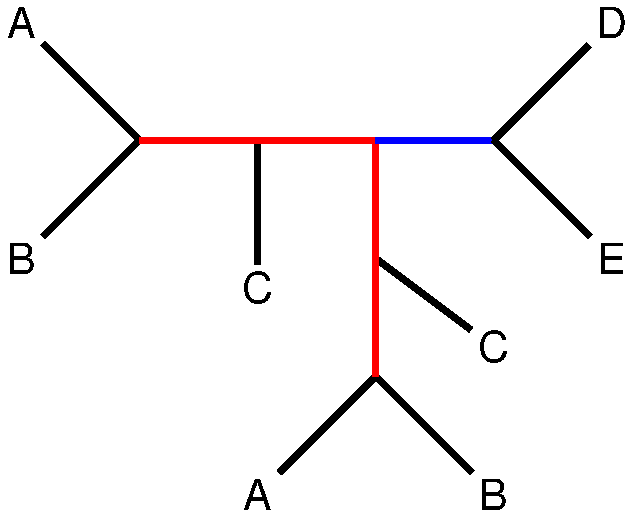
\includegraphics[width=\textwidth]{figures/fastmulrfs-fig1b.pdf}
		~
		\caption{(b) Mul-tree $M$}
	\end{subfigure}
	~~~~~~~~~~~~~~~
	\begin{subfigure}[t]{0.432\textwidth}
		\centering
		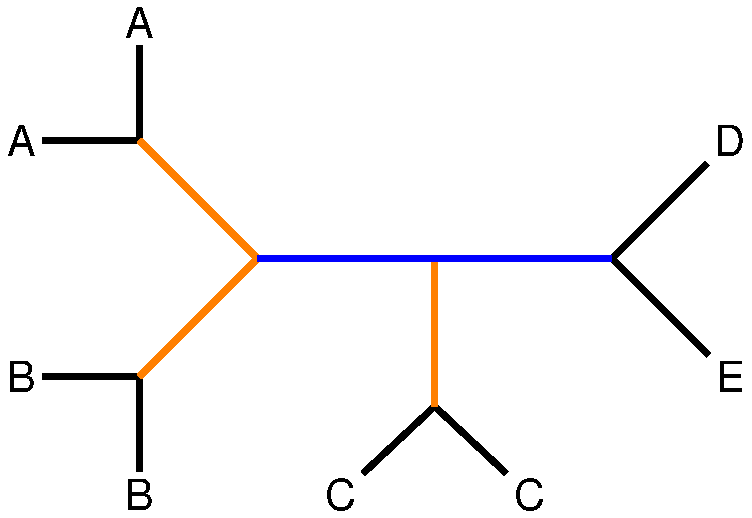
\includegraphics[width=\textwidth]{figures/fastmulrfs-fig1c.pdf}
		~
		\caption{(c) $Ext(T,M)$}
	\end{subfigure}
	
	\vspace{24pt}

	\begin{subfigure}[t]{0.3\textwidth}
		\centering
		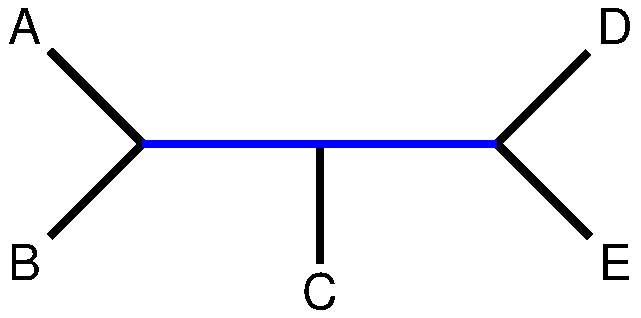
\includegraphics[width=\textwidth]{figures/fastmulrfs-fig1a.pdf}
		~
		\caption{(a) Singly-labeled tree $T$}
	\end{subfigure}
	~~~~
	\begin{subfigure}[t]{0.3\textwidth}
		\centering
		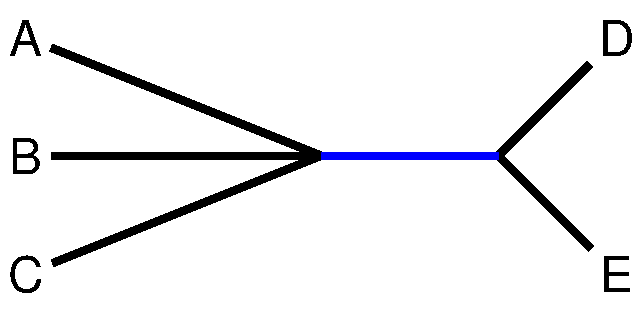
\includegraphics[width=\textwidth]{figures/fastmulrfs-fig1e.pdf}
		~
		\caption{(e) $\mathcal{R}(\mathcal{X}(M))$}
	\end{subfigure}
	~~~~
	\begin{subfigure}[t]{0.3\textwidth}
		\centering
		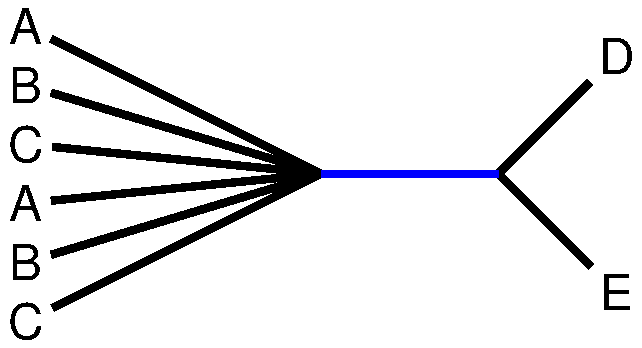
\includegraphics[width=\textwidth]{figures/fastmulrfs-fig1d.pdf}
		~
		\caption{(d) $\mathcal{X}(M)$}
	\end{subfigure}
	\caption{
	{\bf Reduction of the RFS-MUL-trees problem to the RFS problem.}
	Subfigure (a) shows a candidate RFS-MUL-trees supertree $T$ for a set $\mathcal{P}$ of MUL-trees, and subfigure (b) shows a MUL-tree $M$ in ${P}$; note that both $T$ and $M$ are on the same label set $S = \{A, B, C, D, E\}$.
    To compute the RF distance between $T$ and $M$, we build the extended version of $T$ with respect to $M$ (Definition~\ref{defn:extd}), producing $Ext(T,M)$, as shown in subfigure (c).
    The trivial edges in $Ext(T,M)$ (shown in orange) exist in {\em any possible} singly-labeled, binary tree on $S$, so these edges do not impact the solution to the RFS-MUL-trees problem.
    Similarly, the edges in MUL-tree $M$ that are shown in red cannot exist in an extended version of {\em any possible} singly-labeled, binary tree on $S$, so these edges do not impact the solution to the RFS-MUL-trees problem.
   We contract all internal edges in $M$ with the property that there are at least two leaves, one on either side of the edge, with the same label; this produces $\mathcal{X}(M)$, as shown in subfigure (d).
    Furthermore, because all leaves with the same label are now on the same side of {\em every} edge in $\mathcal{X}(M)$, we can delete all but one leaf with each label; this produces $\mathcal{R}(\mathcal{X}(M))$, as shown in subfigure (e).
    The resulting tree is a non-binary, singly-labeled tree on $S$, so we can compute the RF distance between $T$ and $\mathcal{R}(\mathcal{X}(M))$ using Equation~\ref{eq:rf}.
    These observations are formalized in Lemma~\ref{lem:mulrf2}.
    }
	\label{fig:1}
\end{figure}

\subsection{Reducing from MUL-trees to singly-labeled trees}
\label{sec:reduction}
We simplify the RFS-MUL-trees problem by providing an alternative proof that the RF distance between between a singly-labeled tree $T$ and a MUL-tree $M$ can be computed (up to a constant factor that does not depend on $T$) in polynomial time by reducing the MUL-trees to a set of singly-labeled trees; see Figure \ref{fig:1} for intuition behind this proof.

To begin, we define two transformations that can be applied to a MUL-tree $M = (m, S, \phi)$ or to its full differentiation $M' = (m, S', \phi')$ by using the function $f: S' \rightarrow S$ with the property that $f(\phi'(l)) = \phi(l)$ for all $l \in L(m)$.

\begin{definition}[Contracted Version]
\label{defn:conv}
The \emph{\gls{contractedversion}} of $M$, denoted $\mathcal{X}(M)$, is created by contracting every \gls{internaledge} $e$ with the property that there are at least two leaves, one on either side of the edge, with the same label.
Similarly, the contracted version of $M'$, denoted $\mathcal{X}(M')$, is created by contracting every internal edge $e$ with $\pi(e) = A|B$ such that $f(A) \cap f(B) \neq \emptyset$.
\end{definition}

\begin{definition}[Reduced Version]
\label{defn:redv}
If all leaves with species label $s$ are on the same side of {\em every} internal edge in $E(M)$, then they can be represented by a single leaf labeled $s$.
The \emph{\gls{reducedversion}} of $M$ or $M'$, denoted $\mathcal{R}(M)$ or $\mathcal{R}(M')$, respectively, is created as follows. 
For every $s \in S$ with the aforementioned property, delete all but one of the leaves in the set $\{ f(\phi'(l)) = \phi(l) = s : l \in L(m) \}$ (suppressing \glspl{internalnode} of degree 2) and relabel the remaining leaf $s$.
\end{definition}

It is easy to see that $\mathcal{R}(\mathcal{X}(M'))$ is a singly-labeled tree that is isomorphic to $\mathcal{R}(\mathcal{X}(M))$, because after applying the function $\Sigma$ to either $M'$ or $M$, all the leaves with species label $s$ will be on the same side of every edge and thus can be replaced by a single leaf with species label $s$ by applying the function $\mathcal{R}$. 
This observation holds for all $s \in S$.

\begin{lemma}
\label{lem:mulrf2}
Let $T$ be an unrooted, singly-labeled, and \gls{fullyresolved} tree on label set $S$, 
let $M = (m, S, \phi)$ be an unrooted MUL-tree, and
let $Ext(T,M)'$ and $M' = (m, S', \phi')$ be MCFDs of $Ext(T,M)$ and $M$, respectively.
Then,
\begin{equation}
	\label{eq:mulrf2}
	RF(Ext(T,M)', M') = RF(T, M_X) + K
\end{equation}
where $M_X = \mathcal{R}(\Sigma(M))$ and $K$ is a constant that does not depend on the \gls{topology} of the singly-labeled tree $T$ on $S$.
\end{lemma}
\begin{proof}
Let $f: S' \rightarrow S$ be a function with the property that $f(\phi'(l)) = \phi(l)$ for all $l \in L(m)$.
Now we define the following bipartition sets.
\begin{align}
	X &= \{  A|B \in Bip(M') : f(A) \cap f(B) \neq \emptyset \} \\
	R &= \{ A|B \in Bip(M') \setminus X : |A| > 1, |B| > 1, \text{ and either } |f(A)| = 1 \text{ or } |f(B)| = 1 \}
\end{align}
It is easy to see that $X$ contains bipartitions that {\em cannot exist} in $Bip(Ext(T,M)')$ for any singly-labeled tree $T$ on $S$ and that $R$ contains bipartitions that {\em must exist} in $Bip(Ext(T,M)')$ for any singly-labeled tree $T$ on $S$.
(note that edges that induce bipartitions in the set $X$ are colored red in Figure~\ref{fig:1}b and edges that induce bipartitions in the set $R$ are colored orange in Figure~\ref{fig:1}c.)
Let $E'$ denote $Ext(T,M)'$. Then,
\begin{align}
| Bip(E') \cap Bip(M') | &= | Bip(E') \cap Bip(\mathcal{X}(M')) | \\
	&= | Bip(\mathcal{R}(E')) \cap Bip(\mathcal{R}(\mathcal{X}(M'))) | + | R | + |L(m)| - | S | \nonumber  \\
	&= | Bip(T) \cap Bip(M_X) | + | R | + |L(m)| - | S | \nonumber \\
	&= 0.5 \big[ | E(M_X)| + | E(T) | - RF(T, M_X) \big] + | R | + |L(m)| - | S | \nonumber \\
	&= 0.5 \big[ | E(M_X)| + 2 | S | - 3 - RF(T, M_X) \big] + | R | + |L(m)| - | S | \nonumber \\
	&= 0.5 \big[ | E(M_X) | - 3 - RF(T, M_X) \big] + | R | + |L(m)| \nonumber
\end{align}
Let $c$ be the number of species in $S(M)$ that have multiple copies (i.e., $c = | \{ s \in S(M) \}|$). 
Then,
\begin{align}
RF(E', M') &= |E(E') | + |E(M')| - 2| Bip(E') \cap Bip(M') | \\
&= \big( |S| - 3 + c + |L(m)|  \big)  + | E(m) | - 2| Bip(E') \cap Bip(M') | \nonumber \\
&= RF(T, M_X) + |S| + c + | E(m) | - | E(M_X) | - 2 |R| - |L(m)| \nonumber
\end{align}
where $S$, $c$, $E(m)$, $E(M_X)$, $R$, and $L(m)$ are independent of $T$.
\end{proof}

In Lemma~\ref{lem:mulrf2}, we show that $MulRF(Ext(T,M),M)$ can be computed in polynomial time, because computing $RF(Ext(T,M)',M')$ does not depend on the MCFDs of $Ext(T,M)$ and $M$. 
In addition, we show that the RF distance between $Ext(T,M)$ and $M$ can be computed (up to a constant factor that does not depend on the topology of a singly-labeled tree $T$ on $S$) by simply transforming $M$ into a (potentially \gls{unresolved}) singly-labeled tree on $S$ and computing its RF distance from $T$.

The following theorem easily follows from Lemma~\ref{lem:mulrf2}.

\begin{theorem}
\label{thm:equal}
Let $\mathcal{P}$ be a set of unrooted MUL-trees, let $\mathcal{P}_X = \{ \mathcal{R}(\mathcal{X}(M)) : M \in \mathcal{P} \}$, and let $T$ be an unrooted, singly-labeled, and fully resolved tree on label set $S = \bigcup_{M \in \mathcal{P}} S(M)$.
Then, $T$ is an RFS-MUL-trees supertree for $\mathcal{P}$ if and only if $T$ is an RF supertree for $\mathcal{P}_X$.
\end{theorem}

\begin{definition}[Valid and Invalid Bipartitions]
\label{def:valid}
Let $M = (m, S, \phi)$ be an unrooted MUL-tree.
Suppose that deleting an edge $e$ but not its endpoints from $M$ produces two subtrees $m_A(e)$ and $m_B(e)$, defining the label sets: $A  = \{ \phi(l) : l \in L(M_A) \}$ and $B = \{ \phi(l) : l \in L(M_B) \}$.
If $A\cap B = \emptyset$, we say that $e$ induces a \emph{\gls{validbipartition}} and allow $\pi(e) = A|B$ to be contributed to the set $Bip(M)$.
If $A \cap B \ne \emptyset$, we say that $e$ induces an \emph{\gls{invalidbipartition}} and do \emph{not} allow $\pi(e) = A|B$ to be contributed to the set $Bip(M)$; alternatively, we say that $e$ fails to induce a bipartition.
\end{definition}

\begin{theorem}
\label{thm:equal-2}
Let $\mathcal{P}$ be a set of unrooted MUL-trees, and let $T$ be an unrooted, singly-labeled, and fully resolved tree on label set $S = \bigcup_{M \in \mathcal{P}} S(M)$.
By combining Lemma~\ref{lem:mulrf2} and Definition~\ref{def:valid}, it is easy to see that $T$ is in the set:
\begin{equation}
	 \sum_{M \in \mathcal{P}} RF(T|_{S(M)}, M)
\end{equation}
if and only if $T$ is an RFS-MUL-trees supertree for $\mathcal{P}$.
\end{theorem}

\subsection{FastMulRFS}
A consequence of Theorem \ref{thm:equal} is that any heuristic for the RFS problem can be used for the RFS-MUL-trees problem simply by computing $\mathcal{P}_X$ prior to running the heuristic.
In this study, we explore the impact of using FastRFS \cite{vachaspati2015fastrfs}, an effective heuristic for the RFS problem, which solves the bipartition-constrained version of the RFS problem exactly using DP.
We refer to this pipeline as FastMulRFS.
\begin{itemize}
	\item \textbf{\gls{FastMulRFSInput}}: Set $\mathcal{P} = \{M_1, M_2, \dots, M_k\}$ of \gls{unrooted}  \glspl{MUL-tree}
	\item \textbf{\gls{FastMulRFSOutput}}: An unrooted, \gls{fullyresolved} \gls{phylogenetictree} $T$ on label set $S = \bigcup_{i=1}^k S(M_i)$ such that 
	$\sum_{i=1}^k RF(T |_{S(M_i)}, M_i)$ is maximized
	and $Bip(T) \subseteq \Sigma$ (note that $\Sigma$ is a set of allowed \glspl{bipartition} computed from $\mathcal{P}$)
\end{itemize}
The set $\Sigma$ is the space that FastRFS required to run FastRFS, and the current implementation of FastRFS runs ASTRAL-III to compute $\Sigma$. This leads to the following pipeline.

\vspace{12pt}

\begin{algorithm}[!h]
\small
\caption{{\bf FastMulRFS.}}
\label{alg:fastmulrfs}
\setstretch{1.15}
\DontPrintSemicolon
\SetAlgoLined
\SetAlgoNoLine
\LinesNumberedHidden
\SetKwFunction{FastMulRFS}{FastMulRFS}
\SetKwFunction{ASTRAL}{ASTRAL}
\SetKwFunction{FastRFS}{FastRFS}
\SetKwFunction{ContractThenReduceMultree}{ContractThenReduceMultree}
\SetKwProg{Pn}{Function}{:}{}
\SetKwInOut{Input}{Input}
\SetKwInOut{Output}{Output} 
\vspace{.1in}
\Input{Set $\mathcal{P} = \{M_1, M_2, \dots, M_k\}$ of unrooted MUL-trees}
%\vspace{-10pt}
\Output{An unrooted, fully resolved phylogenetic tree $T$ on  $S = \bigcup_{i=1}^k S(M_i)$ s.t. 
	$\sum_{i=1}^k RF(T |_{S(M_i)}, M_i)$ is maximized
	and $Bip(T) \subseteq \Sigma$}
\vspace{-4pt}

\hrulefill
 
\Pn{\FastMulRFS{$\mathcal{P}$}}{
	\vspace{10pt}
	{\bf Step 1:} Use Algorithm~\ref{alg:fastmulrfs-preprocess} to create $\mathcal{P}_X = \{ \mathcal{R}(\mathcal{X}(M)) : M \in \mathcal{P} \}$ in $O(mnk)$ time, where $n = |S|$ and $m$ is the largest number of leaves in any MUL-tree in $\mathcal{P}$.\;
	$\mathcal{P}_X \leftarrow$ \ContractThenReduceMultree{$\mathcal{P}$}\;
	\vspace{10pt}
	{\bf Step 2:} Use ASTRAL-III \cite{zhang2018astral} to produce a set $\Sigma$ of allowed bipartitions s.t. $| \Sigma | = O(nk)$. By {\em default}, $\Sigma$ includes the bipartition set induced by every tree in $M_X \in \mathcal{P}_X$ such that $S(M_X) = S$. Other bipartitions may be added to $\Sigma$ to guarantee at least one fully resolved tree $T$ satisfies $Bip(T) \subseteq \Sigma$ and to improve accuracy by expanding the space of allowed solutions. The running time of ASTRAL-III is $O(nk |\Sigma|^{1.726})$; we run ASTRAL-III to construct $\Sigma$ and then exit.\;
	$\Sigma \leftarrow $\ASTRAL{$\mathcal{P}_X$}\;
	\vspace{10pt}
	{\bf Step 3:} Run FastRFS \cite{vachaspati2015fastrfs} in $O(nk|\Sigma|^2)$ time.\;
	$T \leftarrow$ \FastRFS{$\mathcal{P_X}$, $\Sigma$}\;
	\vspace{10pt}
	\Return{$T$}\;	
 }
\vspace{3pt}
\end{algorithm}

\vspace{6pt}

In summary, FastMulRFS runs in $O(mnk + nk|\Sigma|^2)$ time, where $n$ is the number of species, $k$ is the number of MUL-trees, and $m$ is the largest number of leaves in any of the MUL-trees.
The default technique for constructing the set $\Sigma$ of allowed bipartitions enforces $|\Sigma| = O(nk)$ and as we will show, this suffices for proofs of statistical consistency under generic GDL models when no adversarial GDL occurs.

\subsection{Species Tree Estimation using FastMulRFS}
\label{sec:fastmulrfs}
\paragraph{Generic GDL models:}
Our generic GDL models proceed in the same fashion as the probabilistic \gls{GDL} models proposed by Arvestad {\em et al.} \cite{arvestad2009gene}; however, instead of having one duplication rate $\lambda$ and one loss rate $\mu$ that is fixed across every branch of the species tree and across every gene, we allow each gene $g$ and each edge $e$ to have its own duplication rate $\lambda(e,g)$ and loss rate $\mu(e,g)$; in this way, our generic GDL model is similar to the NCM model.
It is easy to see that our generic GDL models contain the probabilistic GDL models of \cite{arvestad2009gene} as sub-models.
Recall that under these GDL models, duplications and losses follow a Poisson process. 
Let $N(e, g)$ denote the number of events (either duplications or losses) on edge $e$ for gene $g$, and let $t(e)$ denote the length of the edge $e$ in time units.
Then, for gene $g$, the probability of $n$ events on edge $e$ is
\begin{equation}
	P\big(N(e,g) = n\big) = 
	\frac{1}{n!} \bigg( \big( \lambda(e,g) + \mu(e,g) \big) \cdot t(e) \bigg)^n 
	\times exp\bigg(-\big(\lambda(e,g) + \mu(e,g) \big) \cdot t(e) \bigg)
\end{equation}
Clearly, the probability of no duplication/loss events (i.e., $n=0$) is strictly greater than zero for every edge $e$ and every gene $g$.

\paragraph{Adversarial GDL:}
\glsreset{adversarialGDL}
We say that \textit{\gls{adversarialGDL}} has occurred when the gene evolution process produces a gene family tree with a bipartition $\pi$ that is {\em not} \gls{compatible} with the true species tree $T^*$ (Definition~\ref{def:bipartition-compatibility}).
Adversarial GDL requires a sequence of events (a duplication followed by a carefully selected set of losses) that coordinate to produce such a bipartition.
Figure~\ref{fig:2}d illustrates a scenario where adversarial GDL occurs: a gene duplicates on the edge above $Y$, the \gls{MRCA} of species $\{A, B, C\}$, in the species tree (Figure~\ref{fig:2}a), so that $Y$ has two copies of the gene.
Then, one copy of the gene is lost on the edge above $B$, whereas the other copy of the gene is lost on the edge above $A$ and on the edge above $C$.
As a result, the gene family tree shown in Figure \ref{fig:2}d is singly-labeled, but the gene family tree induces a bipartition ($A,C|B,D$) that is incompatible with the species tree; by definition, this is adversarial GDL.

Figure~\ref{fig:2}b illustrates an alternative scenario where the same duplication event is followed by one copy of the gene being lost on the branch above the MRCA of species $\{B, C\}$. 
In this case, not only is there no adversarial GDL, but also the gene family tree induces a bipartition ($A,D|B,C$) that is compatible with the species tree.
Because one of the species retains both copies of a gene, the two arcs that are incident to the duplication node fail to induce bipartitions, as they are on the path between two leaves with the same label.
Furthermore, suppose that $A$, $B$, and $C$ are clades (rather than leaves), then every edge in the two $A$ clades (and the edges on the path connecting the two $A$ clades) would fail to induce a bipartition (assuming no other loss events).
In contrast, every edge in the $B$ clade and the $C$ clade would induce a bipartition that is compatible with the species tree (assuming no other duplication events).

In some sense, duplication events hide bipartitions, while losses (following a duplication event) can reveal bipartitions.
A carefully selected pattern of losses (after the duplication) can result in adversarial GDL (i.e., a particular bipartition $\pi$ that is not in the species tree), but small changes to that pattern may well produce bipartitions that are in the true species tree or are incompatible with $\pi$.
Therefore, while adversarial GDL may occur, it may not have high impact on tree estimation based on the RFS-MUL-trees criterion.

\begin{figure}[!h]
	\centering
	%\includegraphics[width=\textwidth]{figures/fastmulrfs-fig2.pdf}
	\begin{subfigure}[t]{0.4\textwidth}
	\centering
		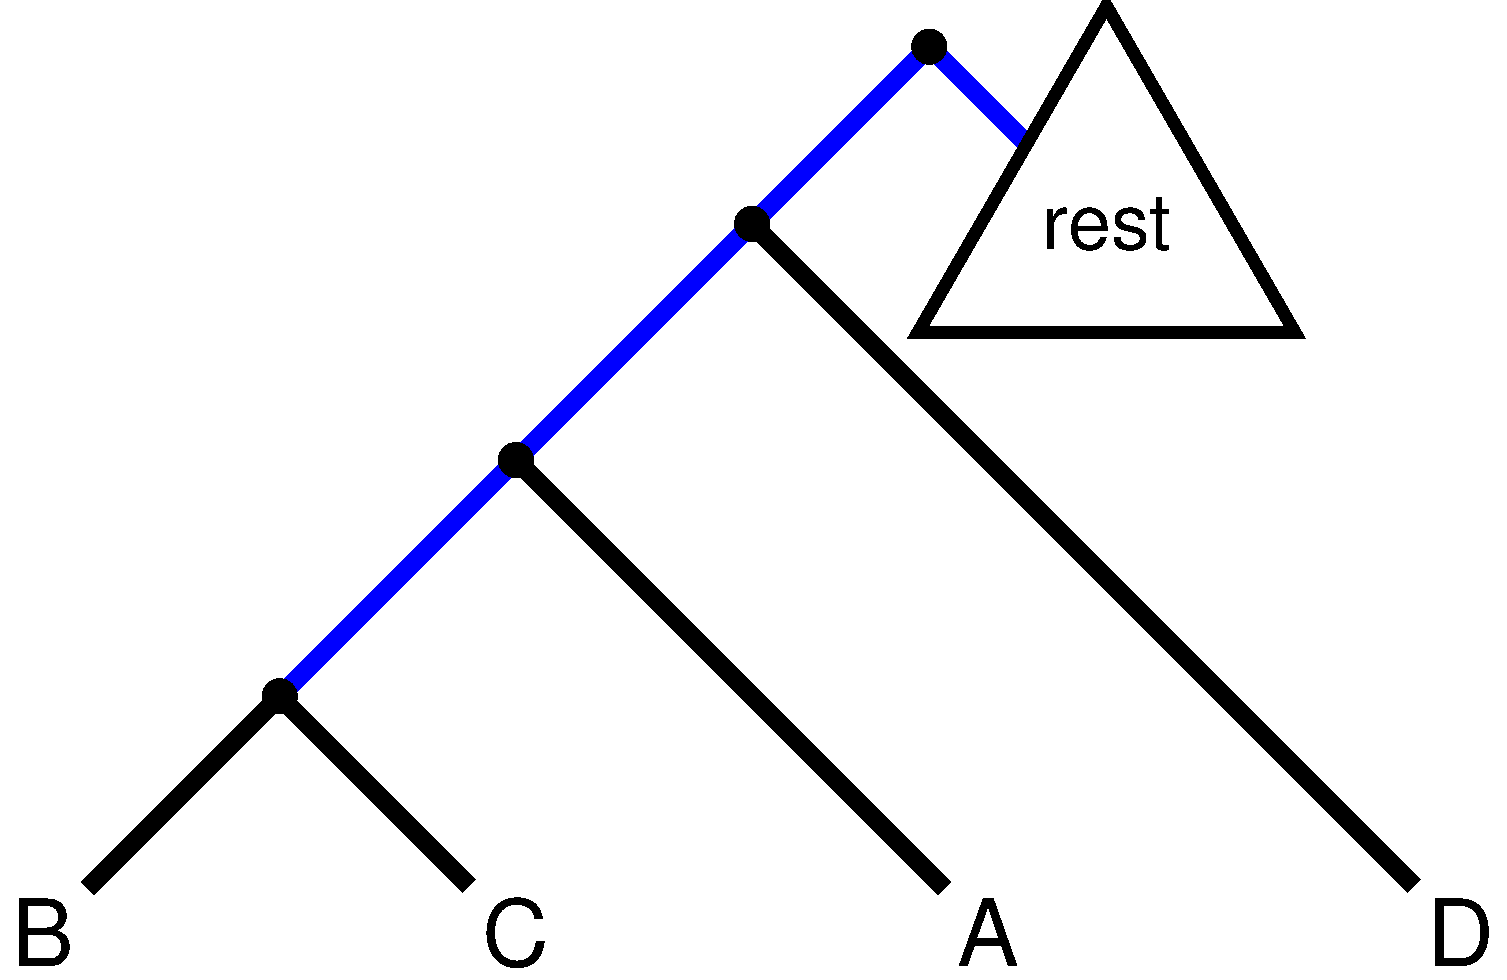
\includegraphics[width=\textwidth]{figures/fastmulrfs-fig2a.pdf}
		~
		\caption{(a) Species tree} 
	\end{subfigure}
	~~~~~~~~~~
	\begin{subfigure}[t]{0.4\textwidth}
	\centering
		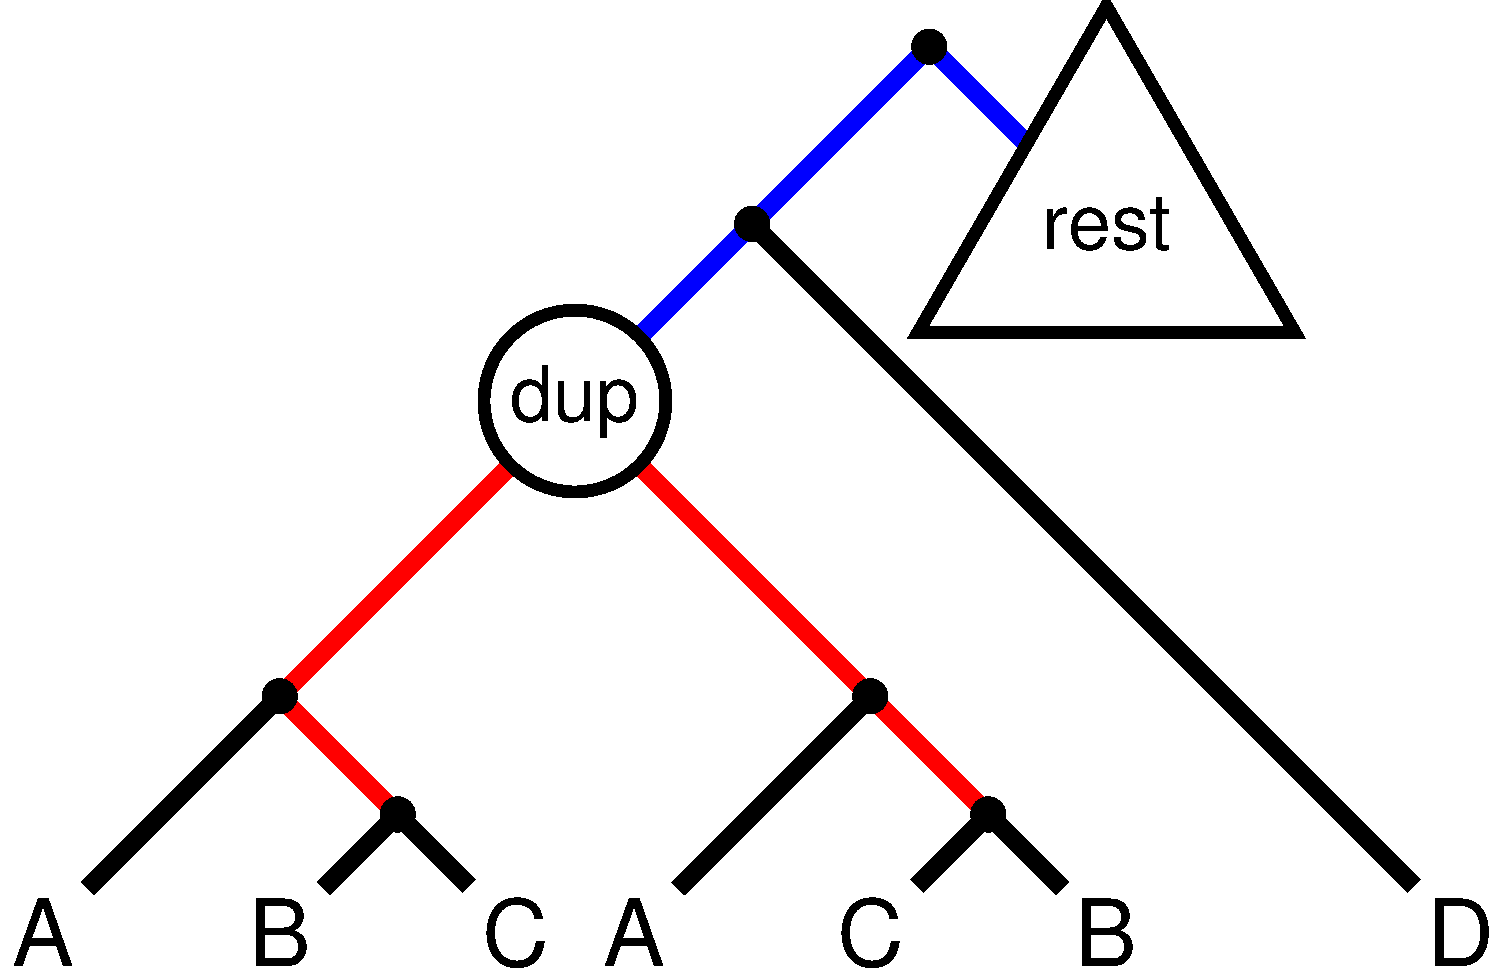
\includegraphics[width=\textwidth]{figures/fastmulrfs-fig2b.pdf}
		~
		\caption{(b) Gene tree: 1 duplication} 
	\end{subfigure}

	\vspace{24pt}

	\begin{subfigure}[t]{0.4\textwidth}
	\centering
		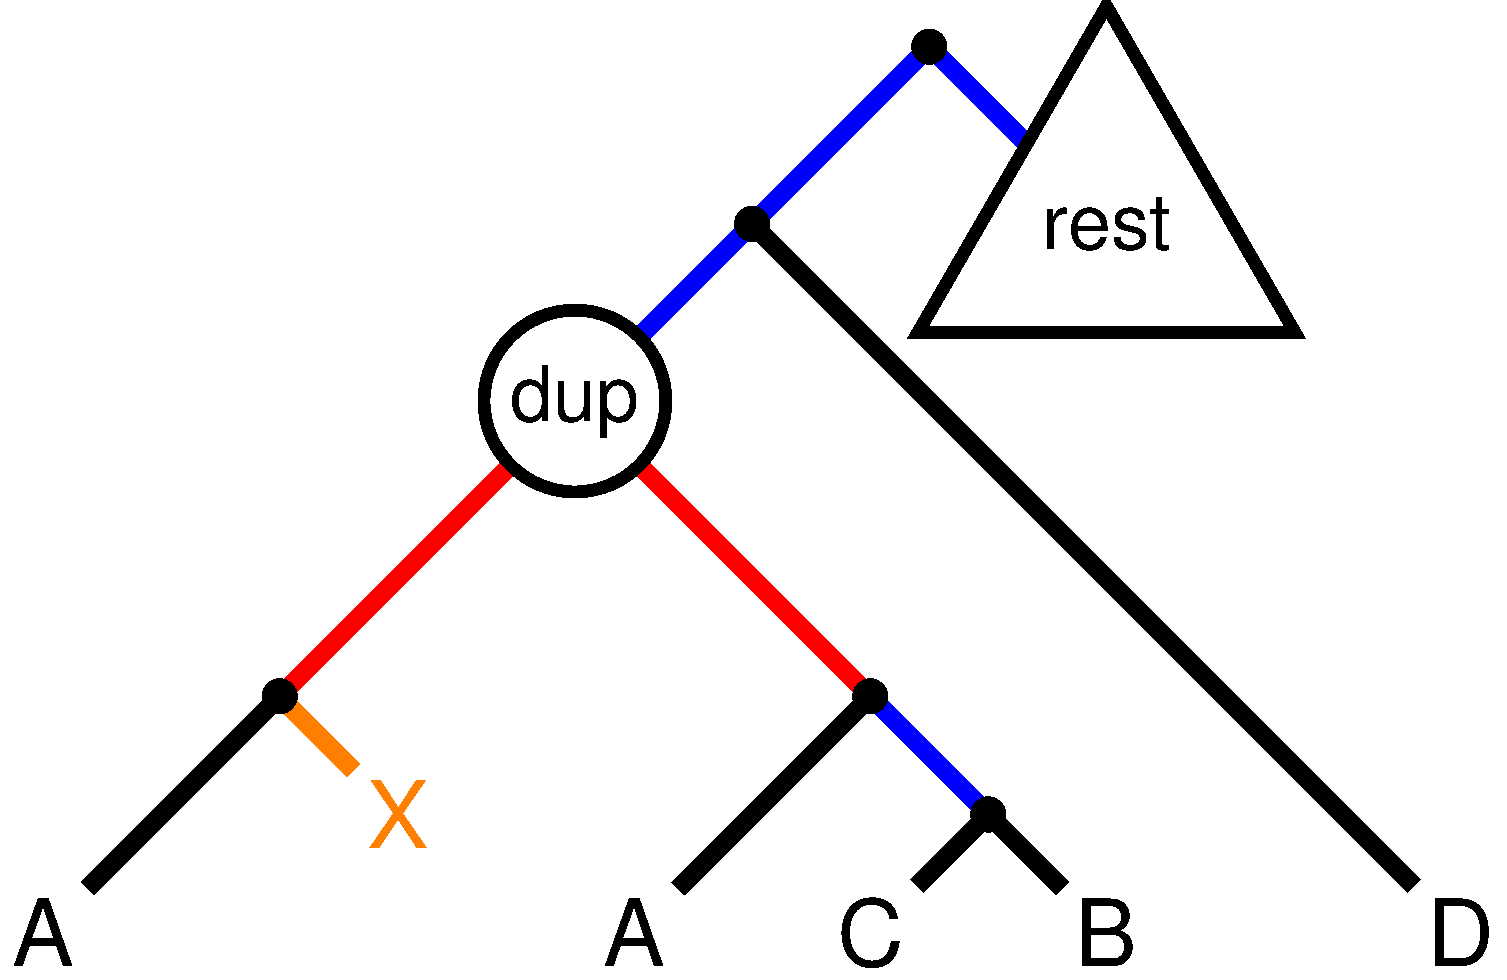
\includegraphics[width=\textwidth]{figures/fastmulrfs-fig2c.pdf}
		~
		\caption{(c) Gene tree: 1 duplication, 1 loss} 
	\end{subfigure}
	~~~~~~~~~~
	\begin{subfigure}[t]{0.4\textwidth}
	\centering
		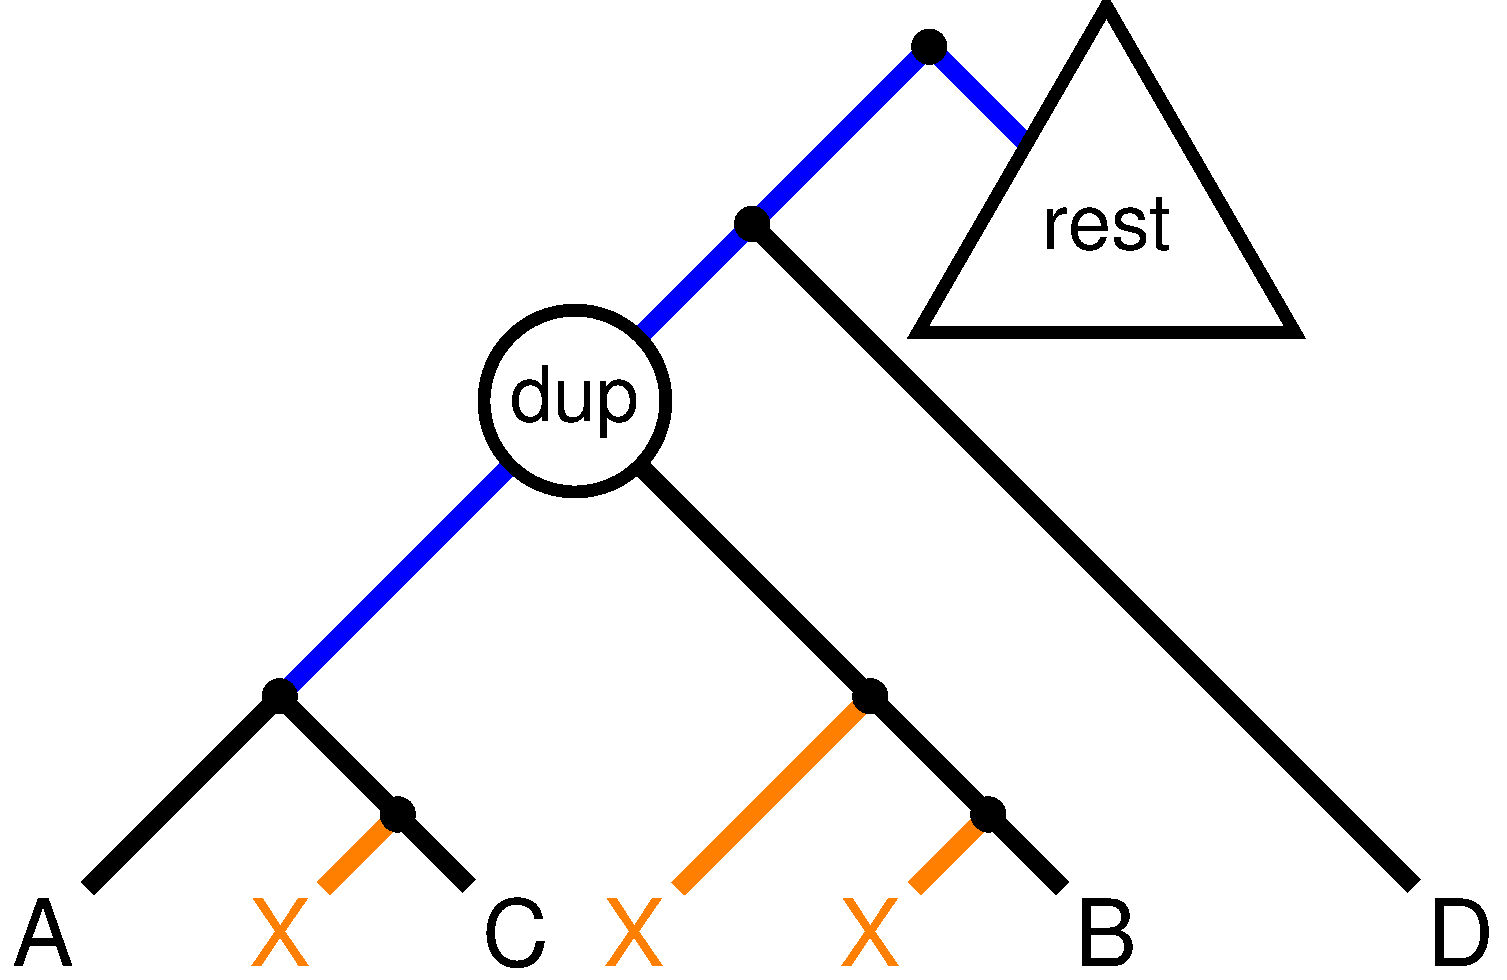
\includegraphics[width=\textwidth]{figures/fastmulrfs-fig2d.pdf}
		~
		\caption{(d) Gene tree: 1 duplication, 3 losses} 
	\end{subfigure}
	\caption{
	{\bf Impact of duplications and losses on RFS-MUL-trees.}
Subfigure (a) shows a rooted species tree and subfigures (b)--(d) show three rooted gene family trees that evolved within the species tree.
Internal edges that induce valid bipartitions are shown in blue, internal edges that induce invalid bipartitions are shown in red, \glspl{terminaledge} are shown in black, and losses are shown in orange.
Subfigure (b) shows a gene family tree with a duplication event on the edge above the MRCA of species $\{ A, B, C \}$, which we refer to as species $Y$. 
All internal edges below the duplication fail to induce bipartitions; therefore, they do not impact the solution space for RFS-MUL-trees.
Subfigure (c) shows a gene family tree with the same duplication event followed by one copy of the gene being lost from the MRCA of species $\{B, C\}$.
Because $A$ retains both copies, the internal edges on the path between $A$ (on the left) and $A$ (on the right) fail to induce bipartitions; therefore, they do not impact the solution space for RFS-MUL-trees.
As long as one species retains both copies of a gene, the two arcs that are incident to the duplication node fail to induce bipartitions, as they must be on the path between two leaves with the same label.
Subfigure (d) shows a gene family tree with the same duplication event followed by one copy of the gene being lost from species $B$ and the other copy of the gene being lost from both species $A$ and $C$.
None of the species that evolved from $Y$ retain both copies of the gene, so all edges below the duplication node induce valid bipartitions.
Because this scenario produces a valid bipartition that is incompatible with the species tree, we refer to this situation as \textit{\gls{adversarialGDL}}. 
	}
	\label{fig:2}
\end{figure}

\clearpage

In the remainder of this section, we will discuss model conditions under which adversarial GDL cannot occur: the {\em duplication-only} case, where all genes evolve with duplication but no loss, and the {\em loss-only} case, where all genes evolve with loss but no duplication.
To prove that a model condition prohibits adversarial GDL, we need to establish that any bipartition that appears in a gene family tree is compatible with the species tree.
Equivalently, any complete bipartition (i.e., a bipartition on the full species set) induced by any gene family tree must also be induced by the species tree, and any incomplete bipartition (i.e., a bipartition on a proper subset of the species set) induced by any gene family tree must be able to be extended (by adding the missing species) so that it becomes a bipartition induced by the species tree (Definition~\ref{def:bipartition-compatibility}).
It is trivial to see that if a gene evolves only with losses, then there is no adversarial GDL for that gene (Lemma \ref{lem:loss}), but the proof for duplication-only evolution is more interesting (Lemma \ref{lem:dup}).

\begin{lemma}
\label{lem:loss}
Let $\mathcal{P}$ be a set of true gene trees that evolved within the rooted species tree $T^*$ under a stochastic loss-only model of gene evolution.
Then, for $\pi \in \{ Bip(M) : M \in \mathcal{P} \}$, $\pi$ is compatible with $T^*$. 
Hence, loss-only models have no adversarial GDL.
\end{lemma}

\begin{lemma}
\label{lem:dup}
Let $\mathcal{P}$ be the set of true gene trees that evolved within the rooted species tree $T^*$ under a stochastic duplication-only model of gene evolution.
Then for every MUL-tree $M \in \mathcal{P}$, $Bip(M) \subseteq Bip(T^*)$.
Hence, duplication-only models have no adversarial GDL.
\end{lemma}

\begin{proof}
Let $M$ be an unrooted version of a MUL-tree in $\mathcal{P}$, and let $e$ be an internal edge in $E(M)$.
We say that an internal edge $e = (x,y) \in E(M)$ lies below a duplication node if there is at least one duplication node on the path from either $x$ or $y$ to the root in the rooted version of $M$; otherwise, we say that $e$ is above all duplication nodes.
An internal edge $e$ is below a duplication node if and only if there is at least one species on both sides of $e$. 
It follows that any internal edge $e$ below a duplication node will be contracted when producing $\mathcal{X}(M)$.
Conversely, an internal edge $e$ is above all duplication nodes if and only if there are no leaves on both sides of $e$ with the same species label.
It follows that any internal edge $e$ above all duplication nodes will {\em not} be contracted when producing $\mathcal{X}(M)$.
Finally, consider a bipartition induced by an edge that is not contracted, and therefore has no duplication nodes above it.
This bipartition appears in the true species tree $T^*$, since the only events that cause the gene family tree to differ from the true species tree are duplications.
\end{proof}

We now prove that FastMulRFS is statistically consistent under generic GDL models if no adversarial GDL occurs.

\begin{theorem}
\label{thm:opt}
The true species tree $T^*$ is an RFS-MUL-trees supertree for any input $\mathcal{P}$ for which no adversarial gene duplication and loss occurred.
\end{theorem}
\begin{proof}
The optimization problem seeks a binary tree $T$ that minimizes the sum of the RF distances to the input MUL-trees; this is equivalent to maximizing the sum of the number of compatible bipartitions in the input MUL-trees. 
If no adversarial GDL occurs, then by definition, every bipartition in the input MUL-trees is compatible with the true species tree $T^*$, and so $T^*$ is an optimal solution to the RFS-MUL-trees problem.
\end{proof}

\begin{theorem}
FastMulRFS is statistically consistent under a generic GDL model for which adversarial GDL is prohibited.
\label{thm:main}

\end{theorem}
\begin{proof}
Let $T^*$ be the true species tree. 
By Theorem \ref{thm:opt}, $T^*$ is an optimal solution to the RFS-MUL-trees problem for any input $\mathcal{P}$ for which no adversarial GDL occurred, so as the number of genes increases, $T^*$ is an optimal solution to the RFS-MUL-trees problem.
FastMulRFS finds an optimal solution to the RFS-MUL-trees problem subject to the output tree $T$ satisfying $Bip(T) \subseteq \Sigma$ (Theorem 3 in \cite{vachaspati2015fastrfs} and Theorem \ref{thm:equal}).
Our generic GDL models assume that the probability of no duplication or loss occurring on an edge is always greater than zero for every gene, so there is a strictly positive probability of the true species tree $T^*$ appearing in the set $\mathcal{P}$ of gene family trees; therefore, as the number of genes increases, $\Sigma$ (as constructed by the default setting within FastMulRFS) will contain all bipartitions in the set $Bip(T^*)$ with probability converging to one.
It follows that, as the number of genes goes to infinity, the probability that FastMulRFS will return $T^*$ converges to one.
\end{proof}

We conclude this section with a conjecture.
\begin{conjecture}
\label{conj:1}
FastMulRFS is statistically consistent under a generic model of GDL for probabilities of gene duplication and loss, so that adversarial GDL has sufficiently low probability.
\end{conjecture}

\section{Performance Study}
\label{sec:fastmulrfs-study}
We evaluated FastMulRFS in comparison to ASTRAL-multi, DupTree, and MulRF on biological and simulated datasets, considering species tree topological accuracy and running time. 

\subsection{Fungal Dataset}
We analyzed a fungal dataset with 16 species and $5\,351$ genes from Rasmussen and Kellis \cite{rasmussen2012unified}, who provided gene family trees estimated from their nucleotide alignments (see Table~\ref{tab:fungi-biological} for an analysis of the number of copies per species in this dataset).
In a prior study, Butler {\em et al.} \cite{butler2009evolution} estimated species trees from this same dataset (specifically the \gls{concatenatedalignment} of putatively orthologous amino acid sequences) using MrBayes \cite{ronquist2003mrbayes}.
The comparison of trees estimated on this biological dataset is difficult to interpret, as the prior concatenation analysis was constrained to enforce the out-grouping of {\em S. castellii} with respect to {\em S. cerevisiae} and {\em C. glabrata}.
Furthermore, the study by Butler {\em et al.} \cite{butler2009evolution} reported several trees that differed with respect to this group (i.e., not all analyses returned this as a clade) as well as with respect to the placement of {\em K. waltii}.
According to their study, none of these resolutions are clearly correct.

\subsection{Simulated Datasets}
\paragraph{Species trees and gene trees:}
We used \gls{SimPhy} version 1.0.2 to simulate a collection of 100-species, 1000-gene datasets under the DLCoal model with six different model conditions: three levels of GDL and two levels of ILS.
The easiest model condition was (largely) based on parameters estimated from the 16-species fungal dataset from Rasmussen and Kellis \cite{rasmussen2012unified} except that we assumed 10 generations per year instead of $1.\bar{1}$ generations per year, which resulted in simulated datasets that were similar to the biological dataset in terms of each species being represented in a similar proportion of gene family trees (Tables~\ref{tab:fungi-biological}--\ref{tab:fungi-simulated}); Supplementary Materials for details.
To make more challenging model conditions, we increased the GDL rate and ILS level by increasing the \gls{EPS}.

We quantified the level of ILS by computing the normalized RF distance between each true \gls{locustree} and its respective true gene tree (which are on the same leaf set), averaging this value across all 1000 locus/gene trees.
The average locus-to-gene tree discord across the 10 replicate datasets was 2\% for the ``no ILS condition'' and 12\% for the ``low/moderate'' ILS condition (note that if we had used 1.1 generations per year, AD would have increased to 19\% and 55\%, respectively).

We also quantified the level of GDL by counting the number of leaves and the number of species per gene tree.
All gene trees had approximately 100 leaves, which is expected since the duplication and loss rates are equal.
As the duplication/loss rate increased, the number of species per gene tree decreased, so even though locus/gene trees had the same number of leaves on average, these leaves were labeled by fewer species.
For duplication/loss rates of $1 \times 10^{-10}$, $2 \times 10^{-10}$, and  $5 \times 10^{-10}$ the average number of species per gene tree was 85, 74, and 53.

We allowed gene trees to deviate from a \gls{strictmolecularclock} by using gene-by-lineage-specific rate heterogeneity modifiers, meaning that for each gene tree, a gamma distribution was defined for each gene tree by drawing $\alpha$ from a log-normal distribution with a location of 1.5 and a scale of one (same parameters as used in \cite{zhang2018astral}), and then each branch length in a gene tree was multiplied by a value drawn the gamma distribution corresponding to that gene tree.

\paragraph{DNA (gene) sequence data:}
We now describe the simulation of DNA sequence data for each gene tree produced by SimPhy.
Again, our protocol is also based on the fungal dataset from Rasmussen and Kellis \cite{rasmussen2012unified}, who provided an estimated \gls{MSA} and an estimated \gls{ML} tree for each of the $5\,351$ genes.
We estimated \gls{GTR+GAMMA} model parameters ($\vec{\pi}$, $Q$, and $\alpha$) for each MSA and ML gene tree pair using \gls{RAxML} version 8.2.12 and then fit distributions to the estimated GTR+GAMMA model parameters (only MSAs with least 500 \gls{parsimony-informative} sites and at most 25\% \glspl{gap} were included in this analysis).
For each gene tree, we drew GTR+GAMMA model parameters from these distributions and then simulated DNA sequences (with 1000 sites) using \gls{INDELible} version 1.03.
Because DNA sequences were simulated without insertions or deletions, MSA estimation was not necessary.

\paragraph{Estimated gene trees:}
ML gene trees were estimated under the GTR+GAMMA model using RAxML version 8.2.12. 
Prior to gene tree estimation, sequences were truncated to the first 25, 50, 100, and 250 nucleotides to produce datasets with varying levels of GTEE.
GTEE was measured by the normalized RF distance between the true and the estimated gene family trees.
Sequence lengths of 25, 50, 100, and 250 resulted in mean GTEE of 67\%, 52\%, 35\%, and 19\%, respectively.

\subsection{Species Tree Estimation}
Finally, species trees were estimated on 25, 50, 100, and 500 gene family trees, either true or estimated, using three different methods: ASTRAL-multi (as implemented in ASTRAL version 5.6.3), DupTree, FastMulRFS (as implemented in release 1.2.0 version 3), and MulRF (as implemented in version 2.1).
All estimated species trees were binary (note that a single optimal tree was taken as an estimate of the species tree even when multiple equally optimal trees were returned by FastMulRFS).
This created $120$ model conditions (three GDL rates, two levels of ILS, five levels of GTEE, and four numbers of genes), each with 10 replicates, for a total of $1\,200$ datasets.

\subsection{Evaluation}
Species tree estimation methods were evaluated in terms of running time and species tree error, as measured by the \gls{RFerrorrate} (Equation~\ref{eq:rf-error}).
All computational experiments were performed on the Campus Cluster at the University of Illinois at Urbana-Champaign, which is a heterogeneous system, meaning that compute nodes can have different specifications (\href{https://campuscluster.illinois.edu/resources/docs/nodes/}{https://campuscluster.illinois.edu/resources/docs/nodes/}).

\section{Results}
\label{sec:fastmulrfs-results}
\subsection{Fungal Dataset}
In an analysis of the fungal dataset, all methods (ASTRAL-multi, FastMulRFS, DupTree, and MulRF) produced species trees that were similar to the MrBayes concatenation tree (Figure \ref{fig:fungi}).
The differences in species trees are minor given the variability in the trees found by Butler {\em et al.} \cite{butler2009evolution}, the use of a topological constraint in their MrBayes analysis, and the uncertainty about the placement of specific taxa in the tree (see Supplementary Information Section 5 in \cite{butler2009evolution} for more information).  

Given that the topological differences are minor and difficult to interpret, we focus on differences in empirical running time.
FastMulRFS and DupTree completed in under a minute each, ASTRAL-multi completed in 18 minutes, and MulRF completed in 40 minutes.
Hence, FastMulRFS is much faster than MulRF and ASTRAL-multi.
While all four of these methods were relatively fast on 16 taxa, we expect the difference between methods to increase on datasets with larger numbers of species and with higher rates of gene duplication.
The improvement in running time over MulRF and ASTRAL-multi is due in part to the fact that both MulRF and ASTRAL-multi use the original gene family trees, while FastMulRFS uses the reduced singly-labeled trees; hence, as the number of leaves or the duplication rate increase, the advantage in running time for FastMulRFS should also increase.

\begin{figure}[!h]
	\centering
	%\includegraphics[width=1.0\textwidth]{figures/fastmulrfs-fig3.pdf}
	\begin{subfigure}[t]{0.31\textwidth}
	\centering
		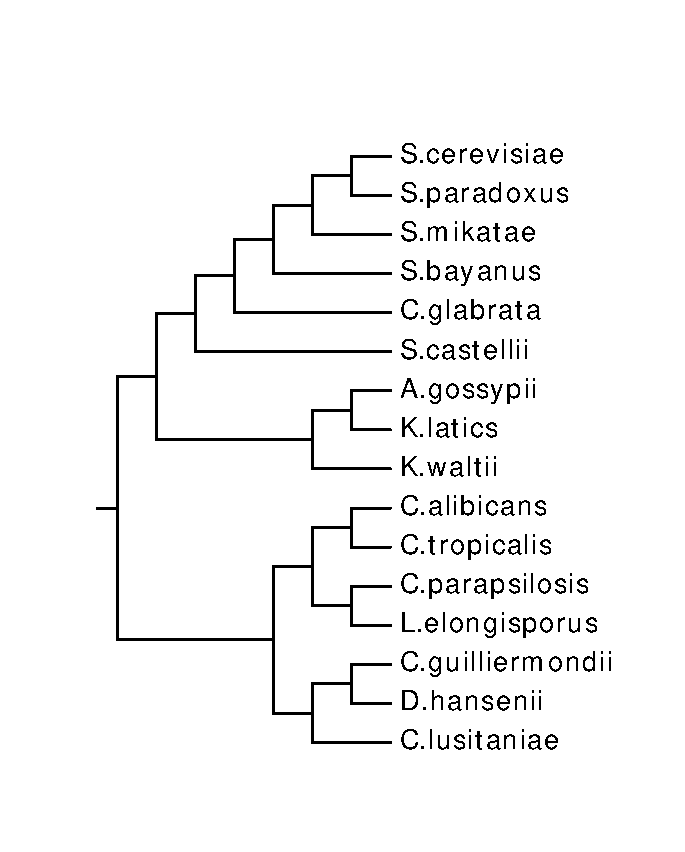
\includegraphics[width=\textwidth]{figures/fastmulrfs-fig3a.pdf}
		\caption{(a) Concatenation} 
	\end{subfigure}
	~
	\begin{subfigure}[t]{0.31\textwidth}
	\centering
		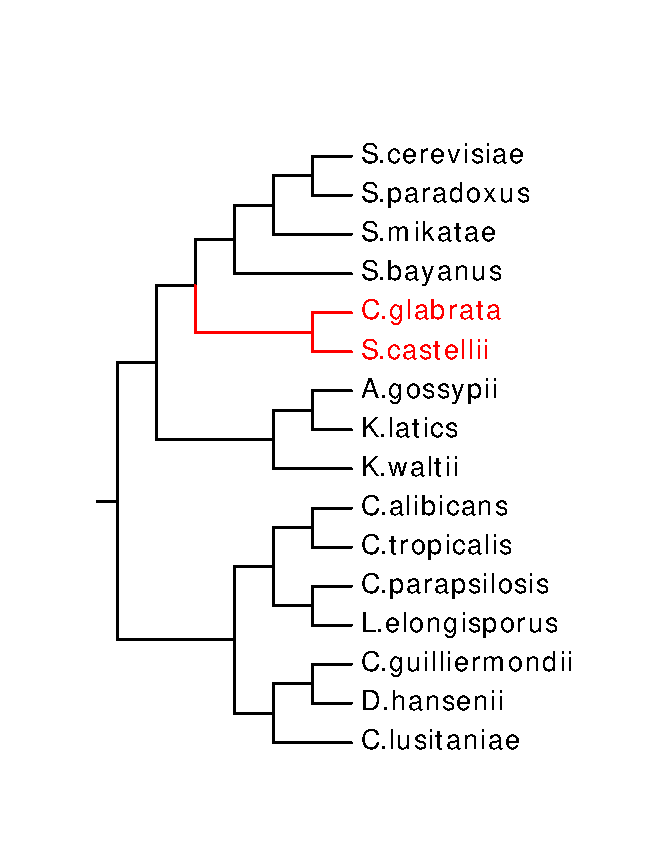
\includegraphics[width=\textwidth]{figures/fastmulrfs-fig3b.pdf}
		\caption{(b) ASTRAL-multi} 
	\end{subfigure}
	~
	\begin{subfigure}[t]{0.31\textwidth}
	\centering
		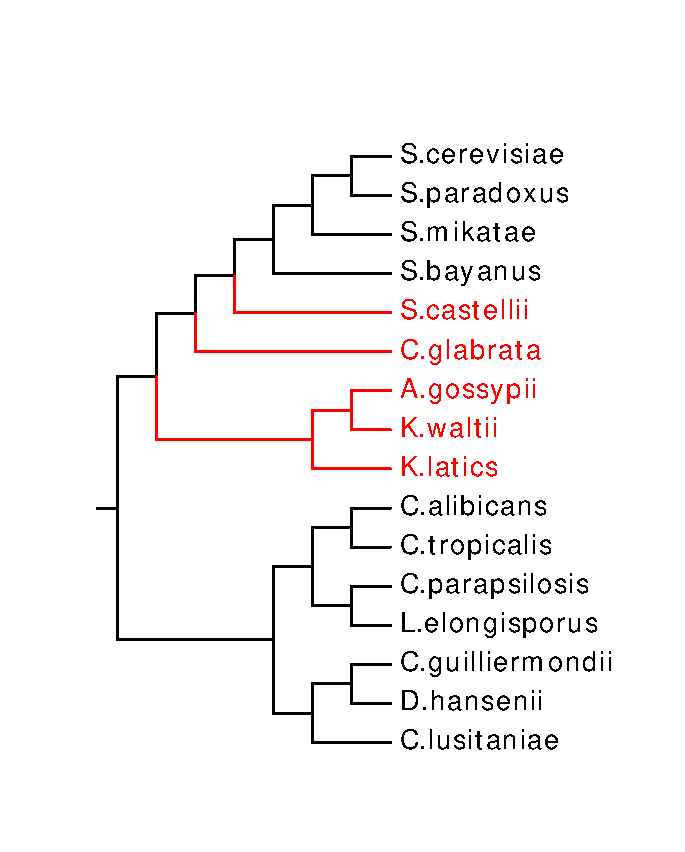
\includegraphics[width=\textwidth]{figures/fastmulrfs-fig3c.pdf}
		\caption{(c) FastMulRFS} 
	\end{subfigure}
   \caption{Species trees were estimated on the 16-taxon fungal dataset with $5\,351$ gene family trees estimated by Rasmussen and Kellis \cite{rasmussen2012unified}. 
   Subfigure (a) shows the MrBayes concatenation tree estimated by Butler {\em et al.} \cite{butler2009evolution}, which is based on putative orthologs instead of the gene family trees.
   Subfigure (b) shows the ASTRAL-multi tree, and subfigure (c) shows the FastMulRFS tree, which is the same tree produced by MulRF and DupTree.
   Topological differences between the MrBayes concatenation tree are highlighted in red; however, this is not indicative of which resolution is correct or incorrect, as the true placement of these taxa is not yet established.
   DupTree and FastMulRFS were the fastest (both completed in less than a minute), ASTRAL-multi estimated a species tree in 18 minutes, and MulRF completed in 40 minutes.}
   \label{fig:fungi}
\end{figure}

\subsection{Simulated Datasets}
DupTree typically had poorer accuracy than the other tested methods (Figures~\ref{fig:fastmulrfs-500gen}--ref{fig:fastmulrfs-100gen}), especially when the level of GTEE was high.
As high GTEE is consistent with the generally low bootstrap branch support values reported for several multi-locus datasets (Table \ref{tab:include-1}), we focus on comparing MulRF, FastMulRFS, and ASTRAL-multi.
All methods improved in accuracy with larger numbers of genes and degraded in accuracy with higher GTEE levels, ILS levels, and/or GDL rates.
The relative accuracy between methods was consistent across all model conditions, although the degree of difference depended on the model conditions, with bigger differences for smaller numbers of genes and higher GTEE levels, ILS levels, and GDL rates.
When given 500 gene trees, error levels were low and differences between methods were (usually) small, so that the main difference was running time.
The fastest method was FastMulRFS, MulRF was the slowest, and ASTRAL-multi was intermediate.

\paragraph{FastMulRFS vs.~MulRF:}
FastMulRFS and MulRF are both heuristics for the RFS-MUL-trees problem.
They were essentially tied for accuracy across all tested conditions (Figures~\ref{fig:fastmulrfs-500gen}--\ref{fig:fastmulrfs-100gen} and Table \ref{tab:fastmulrfs-error}), but FastMulRFS was dramatically faster than MulRF (Figures~\ref{fig:fastmulrfs-500gen}--\ref{fig:fastmulrfs-100gen} and Table \ref{tab:fastmulrfs-rt}). In addition, FastMulRFS nearly always returned a tree with an equivalent or better RFS-MUL-trees score than MulRF. Out of the $1\,200$ datasets analyzed, FastMulRFS was worse than MulRF on 56 datasets, FastMulRFS was equal to MulRF on  962 datasets, and FastMulRFS was better than MulRF on 182 datasets.

\paragraph{FastMulRFS vs.~ASTRAL-multi:}
FastMulRFSwas always at least as accurate on average as ASTRAL-multi (and was often more accurate on average  than ASTRAL-multi) across all model conditions tested (Figures~\ref{fig:fastmulrfs-500gen}--\ref{fig:fastmulrfs-100gen} and Table \ref{tab:fastmulrfs-error}), with larger differences between methods for the higher GTEE conditions and smaller differences for the lower GTEE conditions.
The running times for ASTRAL-multi and FastMulRFS increased with the number of genes, but FastMulRFS was always faster (Figures~\ref{fig:fastmulrfs-500gen}--\ref{fig:fastmulrfs-100gen} and Table \ref{tab:fastmulrfs-rt}).
For example, on the 500-gene model conditions, FastMulRFS typically completed in one to two minutes (and always in under five minutes), whereas ASTRAL-multi used between 10 minutes and 1.2 hours.

\section{Discussion}
To date, only two types of methods have been proven statistically consistent under any GDL model.
The first type of method is based on maximizing quartets that are induced by the gene family trees, and the second type of method  is based on maximizing bipartitions that are induced by the gene family trees.
ASTRAL-multi is an example of the first kind of method, and FastMulRFS is an example of the second type of method; notably, both methods use DP to solve their optimization problems exactly within a constrained search space.
The conditions under which these two methods have been proven statistically consistent are different. 
ASTRAL-multi is established to be consistent under a gene evolution model that requires that all the genes evolve {\em i.i.d.}~within the species tree.
Since the time of our study, Markin and Eulenstein \cite{markin2020quartet} showed that a related quartet-based approach is statistically consistent under the DLCoal model, which allows for both GDL and ILS but still assumes that genes evolve {\em i.i.d.}~within the species tree.
In contrast, FastMulRFS has been proven consistent under a generic model that does not require the genes to evolve {\em i.i.d.}~and indeed allows for a very generic model similar to the NCM model.
This is a relative strength of FastMulRFS, as genes do not evolve {\em i.i.d.}~within a species tree, as discussed in \cite{dondi2019reconciling}.
On the other hand, FastMulRFS has only been proven consistent when no adversarial GDL occurs and no ILS occurs; this is a relative weakness of FastMulRFS (although see Conjecture \ref{conj:1} regarding adversarial GDL).
Therefore, from a theoretical perspective, there are advantages and disadvantages for both methods.

In terms of empirical performance, FastMulRFS was more accurate and more robust to GTEE than ASTRAL-multi under most model conditions we examined.
The only conditions in which the two methods achieved similar accuracy were characterized by low GTEE and large numbers of genes, where both methods achieved very high accuracy.
FastMulRFS also was much faster than ASTRAL-multi, with large improvements in speed for large numbers of genes and high GTEE.
In summary, FastMulRFS had superior performance compared to ASTRAL-multi in our experimental evaluation.

A comparison between FastMulRFS and MulRF is also interesting.
Both methods attempt to solve the same NP-hard optimization problem, and neither is guaranteed to find an optimal solution. 
However, FastMulRFS is guaranteed to find an optimal solution within a constrained search space in polynomial time; furthermore, the way that FastMulRFS constrains its search space is sufficient to ensure that it is statistically consistent.
MulRF, in contrast, uses a locally optimal search strategy combined with hill climbing, so it does not run in polynomial time and may not be provably statistically consistent.
In our experimental study, the two methods were very close in accuracy, but FastMulRFS was dramatically faster. 
Overall, FastMulRFS was superior to MulRF.

FastMulRFS matched or improved on the other methods under all conditions we explored, where gene trees evolved under a unified model of ILS and GDL (which did not prohibit adversarial GDL).
Our study suggests that FastMulRFS may have good robustness and high accuracy, even under conditions where it has not (yet) been proven statistically consistent. 
(note that we think it is unlikely that FastMulRFS is statistically consistent under conditions with high ILS.)
Future work is clearly needed to evaluate FastMulRFS and other methods under a wider range of model conditions, including explicit conditions where adversarial GDL and high levels of ILS occur.
Simulations should also be performed to evaluate other scenarios that produce multi-copy genes, for example whole genome duplication events, which impact species tree estimation for many major clades, including fungi \cite{butler2009evolution} and plants \cite{leebensmack2019one}.
More complex simulations also should be performed (including gene conversion and HGT) in order to better understand the conditions in which methods perform well. 
Along these lines, it would be helpful to characterize biological datasets to understand realistic levels of ILS and GDL (including the frequency of adversarial GDL); this task has been identified as an important challenge throughout this dissertation. 

A limitation of this study is that we examined only a few methods, and future studies should evaluate other methods, including {\em guenomu} (discussed earlier) and MixTreEM \cite{ullah2015species-mixtrem}, to discover the places in the parameter space of model species trees where each method outperforms the others.
Furthermore, methods that operate by making predictions of orthology could be used in a three-phase approach: given inputs with sequence alignments and MUL-trees, predict orthology, reduce to datasets with just orthologous genes (and hence singly-labeled gene trees), and then run a preferred species tree estimation method. 
For example, in a recent preprint, Zhang {\em et al.} \cite{zhang2020astral-pro} presented A-PRO, another modification of ASTRAL, and proved that it is statistically consistent under a GDL model if given correctly ``tagged" gene trees (i.e., each node in each gene tree is correctly identified as either a duplication or not); however, this assumption means that orthology can be inferred without error (an assumption that is not made for ASTRAL-multi).
Studies evaluating A-PRO and these other approaches under a variety of conditions would enable biologists to select methods with the best expected accuracy for their datasets.

While we have focused on the estimated species topology, biologists require that branches in the topology to be annotated with information about the support for or confidence in each branch.
Our reduction on MUL-trees (which transforms them into singly-labeled trees) is useful not only for estimating species trees but also for interpreting estimated species trees.

First, the reduction allows the branches of the species tree to be annotated by the proportion of MUL-trees that contain that branch; this metric is easy to interpret and therefore highly useful.
Second, by combining the reduction with DP in a constrained search space, we can use an existing tool, called SIESTA \cite{vachaspati2017enhancing}, to quantify the space of optimal solutions; specifically, SIESTA reports the number of optimal solutions in the constrained search space and annotates each branch by the proportion of optimal solutions that contain that branch.
This seems especially useful in the context of duplication and loss, as the reduction on MUL-trees illustrates that the MUL-trees are likely to be unresolved when duplications occur; this combined with losses could result in a large space of optimal solutions.

Third, after applying the reduction to MUL-trees, it possible to determine the relative weight of each MUL-tree when solving the RFS-MUL-trees problem.
A MUL-tree $M$ that evolves with only a duplication at a leaf induces $S(M) - 3$ valid bipartitions; however, a MUL-tree that evolves with only a duplication at the root induces zero valid bipartitions; therefore, the output tree could be biased towards a small subset of MUL-trees that contain a disproportionately large number of valid bipartitions compared to the other MUL-trees in the input set.
While this is not a problem in theory, it can be a problem in practice, as MUL-trees can differ from the species tree due to estimation error and other sources of heterogeneity.
This has already been shown to be an issue in the context of ILS.
As an example, gene trees with different numbers of species induce different numbers of quartets, and in this case, each gene tree contributes a different number of quartets to the MQSS problem (which ASTRAL solves within a constrained search space).
Two recent studies \cite{gatesy2017resolving-pcs, gatesy2019partitioned} showed that the resolution of some controversial branches can change by removing outlier gene trees that contribute a disproportionately large number of quartets compared to the other gene trees in the input set.
The ability to recognize that two fully resolved MUL-trees can contribute very different numbers of bipartitions to the RFS-MUL-trees problem is critical for identifying systematic biases, and we hope the theoretical observations of our study further enable the interpretation of species trees estimated from gene family trees.

\section{Conclusions}
\label{sec:conclusions}
We presented FastMulRFS, a new method for estimating species tree from unrooted gene family trees, without needing to have any information about orthology.
FastMulRFS runs in polynomial-time and is provably statistically consistent under a generic GDL when adversarial GDL does not occur.
Prior to our study, the only method established to be statistically consistent under any GDL model was ASTRAL-multi (their proof does assume that genes evolve {\em i.i.d.}~within the species tree but does not prohibit adversarial GDL).
Of course, statistical consistency does not predict performance on finite amounts of data or in the context of model violations (which are perhaps certain to occur when analyzing biological datasets).
In our simulation study, FastMulRFS compared quite favorably (in terms of accuracy and running time) to ASTRAL-multi as well as MulRF.
This is significant as we evaluated methods under conditions where neither FastMulRFS nor ASTRAL-multi are (yet) proven to be statistically consistent. 
Specifically, our proof establishes statistical consistency (of FastMulRFS) under models where ILS, GTEE, or adversarial GDL are prohibited, whereas our study benchmarks methods on datasets simulated with two ILS levels, five GTEE levels, and three GDL rates (note that adversarial GDL was not explicitly prohibited).
Although accuracy is difficult to evaluate on biological datasets, FastMulRFS produced trees that were similar to those produced by other methods and did not violate known relationships.
Overall, the recent advances in development of statistically consistent methods for species tree estimation under GDL models is exciting, and the good performance of many of these methods under a range of model conditions suggests that novel combinations and ideas may lead to even better methods that provide improved accuracy and scalability.

\clearpage

\section{Plots}
\label{sec:fastmulrfs-plots}
This section contains the four plots presented in Section~\ref{sec:fastmulrfs-results} Results. 

\vspace{12pt}

\begin{figure}[!h]
\centering
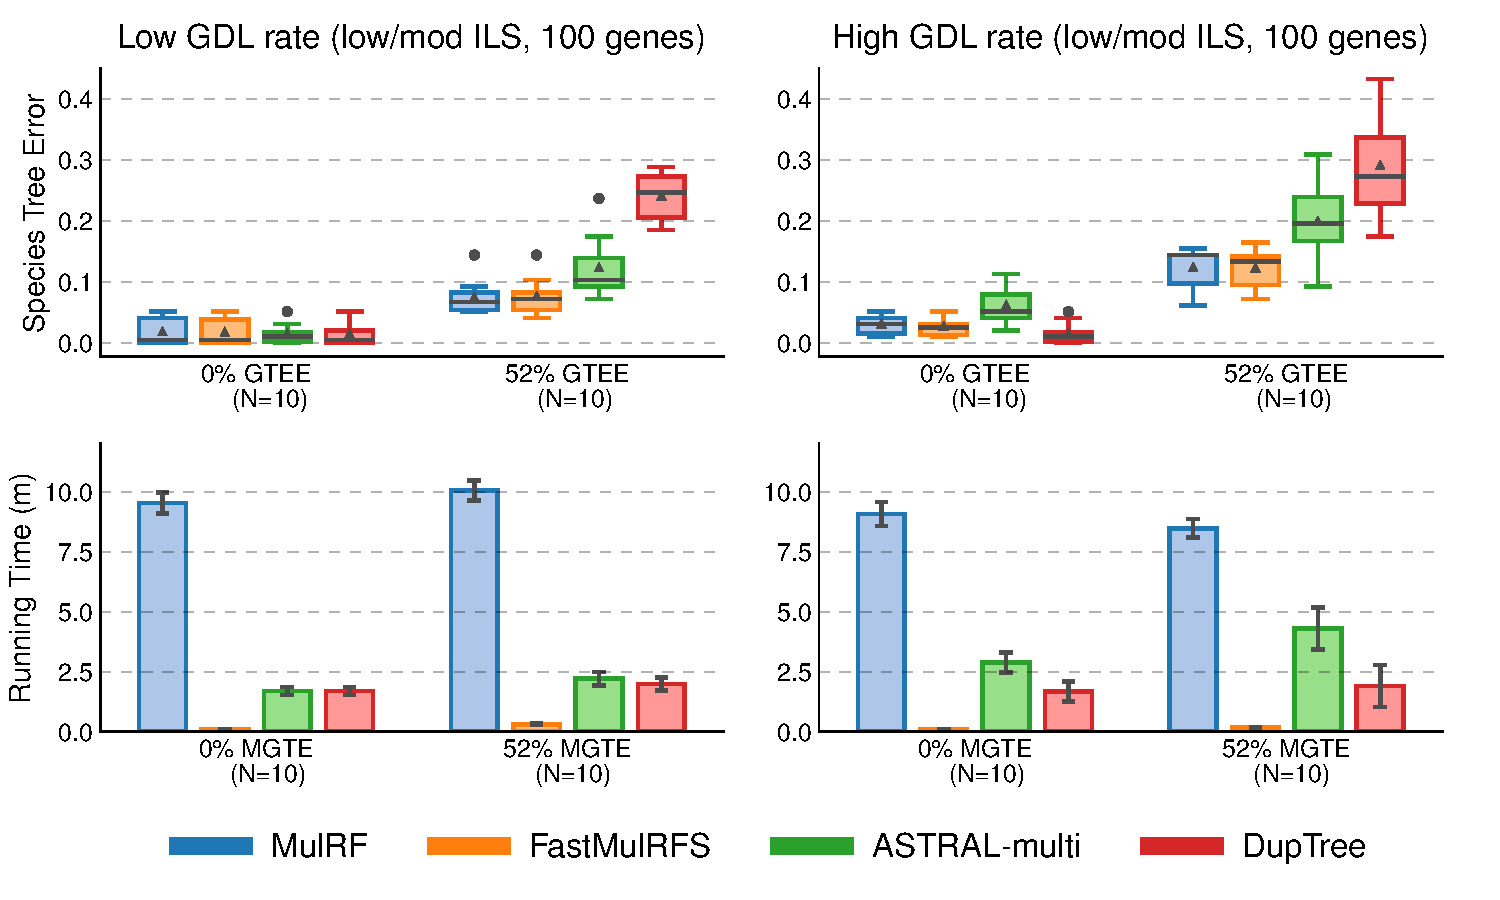
\includegraphics[width=\textwidth]{figures/fastmulrfs-fig4.pdf}
	\caption{{\bf Comparison of species tree estimation methods on 500 gene datasets with low/moderate ILS.} 
	MulRF (blue), FastMulRFS (orange), ASTRAL-multi (green), and DupTree (red) are compared on 100-species, 500 gene datasets with low/moderate ILS (12\%), two levels of GTEE, and two GDL rates (lowest and highest).
	Subplots in the top row show species tree error (RF error rate).
Gray bars represent medians, gray triangles represent means, gray circles represent outliers, box plots are defined by quartiles (extending from the first to the third quartiles), and whiskers extend to plus/minus 1.5 times the interquartile distance (unless greater/less than the maximum/minimum value).
Subplots in the bottom row show running time (in minutes); bars represent means and error bars represent standard deviations across replicate datasets.).
The number $N$ of replicates on which the methods completed is shown on the $x$-axis.}
\label{fig:fastmulrfs-500gen}
\end{figure}

\begin{figure}[!h]
	\centering
	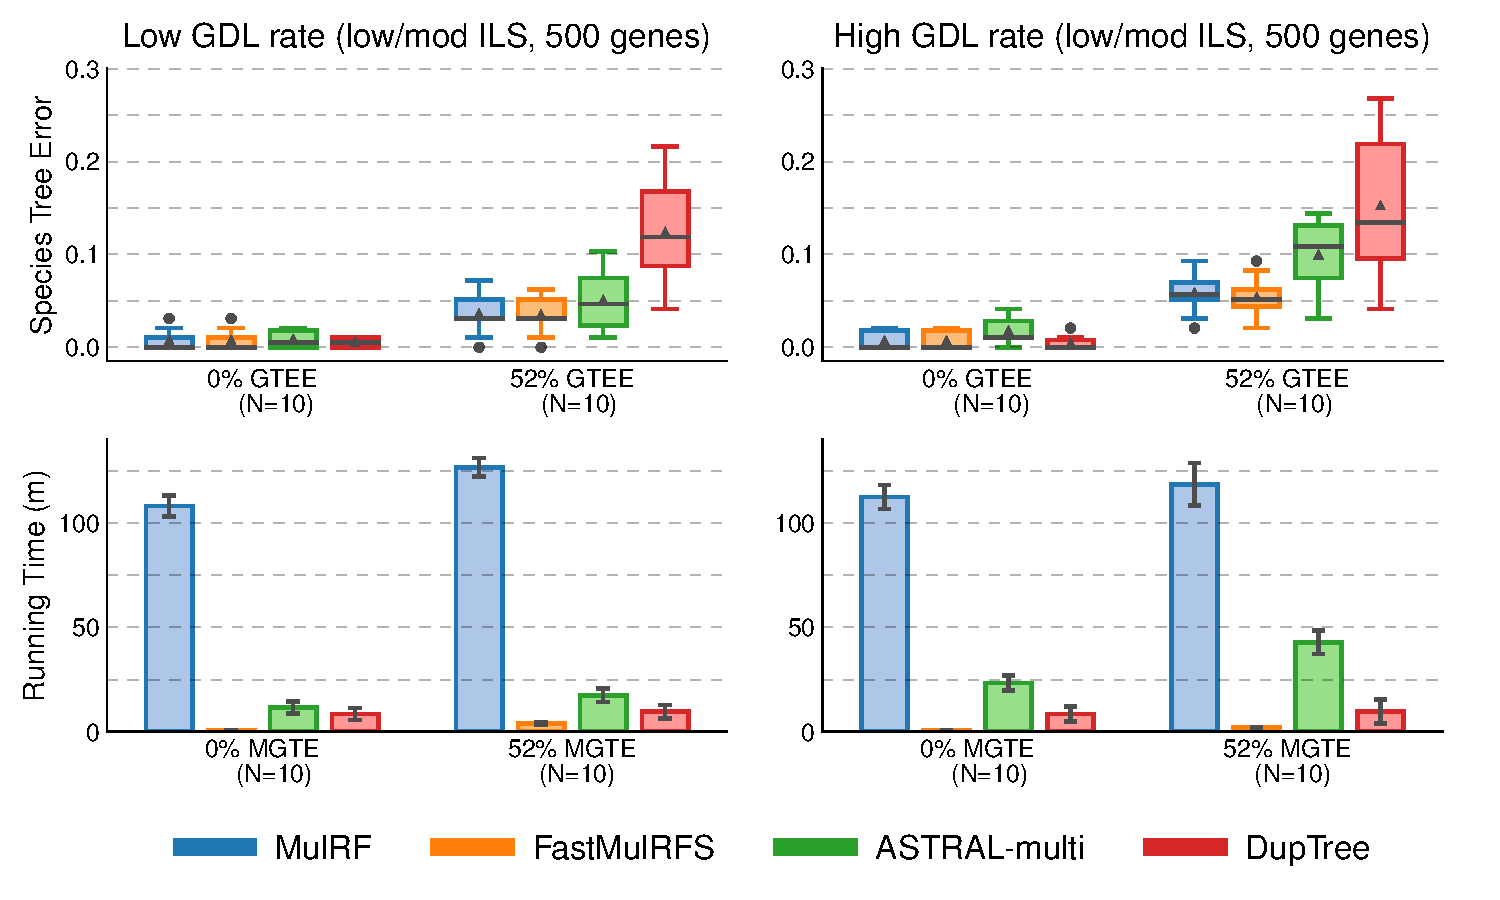
\includegraphics[width=\textwidth]{figures/fastmulrfs-fig5.pdf}
	\caption{{\bf Comparison of species tree estimation methods on 100 gene datasets with low/moderate ILS.} 
	MulRF (blue), FastMulRFS (orange), ASTRAL-multi (green), and DupTree (red) are compared on 100-species, 100 gene datasets with low/moderate ILS (12\%), two levels of GTEE, and two GDL rates (lowest and highest).
	Subplots in the top row show species tree error (RF error rate).
Gray bars represent medians, gray triangles represent means, gray circles represent outliers, box plots are defined by quartiles (extending from the first to the third quartiles), and whiskers extend to plus/minus 1.5 times the interquartile distance (unless greater/less than the maximum/minimum value).
Subplots in the bottom row show running time (in minutes); bars represent means and error bars represent standard deviations across replicate datasets.).
The number $N$ of replicates on which the methods completed is shown on the $x$-axis.}
\label{fig:fastmulrfs-100gen}	
\end{figure}

\clearpage

\section{Tables}
\label{sec:fastmulrfs-tables}
This section contains the two tables presented in Section~\ref{sec:fastmulrfs-study} Performance Study and the two tables presented in \ref{sec:fastmulrfs-results} Results. 

\vspace{12pt}

\begin{table}[!h]
\centering
\setlength{\tabcolsep}{6pt}
%\footnotesize
\caption{{\bf Statistics on the number of copies of each species in the fungal datasets.} 
For the fungal biological dataset, we computed the mean ($\pm$ standard deviation), the minimum, and the maximum number of copies of each species across $5\,351$ gene trees.
We also report the proportion of gene family trees with more than 1, 2, 5, 10, and 20 copies of a species; for example, $>1$ indicates the proportion of gene family trees (out of $5\,351$) with greater than one copy of the species.
}\label{tab:fungi-biological}
\begin{tabular}{ccccc ccccc}
\toprule
Species & Mean $\pm$ Std & Min & Max & $=$1 & $>$1 & $>$2 & $>$5 & $>$10 & $>$20\\
\midrule
 A. gossypii & 0.85 $\pm$ 0.58 & 0 & 13 & 0.731 & 0.050 & 0.008 & 0.001 & 0.000 & 0.000\\
 C. alibicans & 1.04 $\pm$ 0.65 & 0 & 7 & 0.769 & 0.111 & 0.027 & 0.001 & 0.000 & 0.000\\
 C. glabrata & 0.93 $\pm$ 0.81 & 0 & 27 & 0.667 & 0.110 & 0.019 & 0.002 & 0.001 & 0.000\\
 C. guilliermondii & 0.99 $\pm$ 0.70 & 0 & 11 & 0.722 & 0.110 & 0.027 & 0.001 & 0.000 & 0.000\\
 C. lusitaniae & 0.95 $\pm$ 0.62 & 0 & 10 & 0.728 & 0.098 & 0.019 & 0.000 & 0.000 & 0.000\\
 C. parapsilosis & 1.00 $\pm$ 0.73 & 0 & 12 & 0.729 & 0.110 & 0.028 & 0.003 & 0.000 & 0.000\\
 C. tropicalis & 1.04 $\pm$ 0.73 & 0 & 8 & 0.738 & 0.122 & 0.033 & 0.003 & 0.000 & 0.000\\
 D. hansenii & 1.02 $\pm$ 0.65 & 0 & 7 & 0.756 & 0.110 & 0.026 & 0.002 & 0.000 & 0.000\\
 K. latics & 0.89 $\pm$ 0.63 & 0 & 15 & 0.745 & 0.063 & 0.010 & 0.002 & 0.000 & 0.000\\
 K. waltii & 0.88 $\pm$ 0.71 & 0 & 18 & 0.736 & 0.059 & 0.011 & 0.002 & 0.001 & 0.000\\
 L. elongisporus & 0.98 $\pm$ 0.66 & 0 & 9 & 0.727 & 0.108 & 0.021 & 0.001 & 0.000 & 0.000\\
 S. bayanus & 0.94 $\pm$ 0.81 & 0 & 23 & 0.643 & 0.128 & 0.022 & 0.002 & 0.000 & 0.000\\
 S. castellii & 1.01 $\pm$ 0.91 & 0 & 25 & 0.638 & 0.154 & 0.028 & 0.003 & 0.001 & 0.000\\
 S. cerevisiae & 1.03 $\pm$ 1.09 & 0 & 42 & 0.678 & 0.141 & 0.027 & 0.004 & 0.001 & 0.001\\
 S. mikatae & 0.92 $\pm$ 0.76 & 0 & 18 & 0.646 & 0.118 & 0.021 & 0.002 & 0.000 & 0.000\\
 S. paradoxus & 0.95 $\pm$ 0.83 & 0 & 25 & 0.649 & 0.129 & 0.023 & 0.002 & 0.000 & 0.000\\
\bottomrule
\end{tabular}
\end{table}

\clearpage

\begin{table}[!h]
\centering
\setlength{\tabcolsep}{4pt}
%\footnotesize
\caption{{\bf Statistics on the number of copies of each species in the datasets simulated based on the fungal dataset.} This is the same as Table~\ref{tab:fungi-biological} but data for the first 15 species in the first replicate datasets are shown.}
\label{tab:fungi-simulated}
\begin{tabular}{ccccc ccccc}
\toprule
Species & Mean $\pm$ Std & Min & Max & $=$1 & $>$1 & $>$2 & $>$5 & $>$10 & $>$20\\
\midrule
\multicolumn{10}{l}{\em Assuming 10 generations per year}\\[0.5ex]
 1 & 1.02 $\pm$ 0.57 & 0 & 4 & 0.743 & 0.128 & 0.021 & 0.000 & 0.000 & 0.000\\
 2 & 1.01 $\pm$ 0.60 & 0 & 4 & 0.703 & 0.144 & 0.018 & 0.000 & 0.000 & 0.000\\
 3 & 0.99 $\pm$ 0.56 & 0 & 5 & 0.736 & 0.119 & 0.012 & 0.000 & 0.000 & 0.000\\
 4 & 1.01 $\pm$ 0.60 & 0 & 4 & 0.703 & 0.142 & 0.019 & 0.000 & 0.000 & 0.000\\
 5 & 1.01 $\pm$ 0.61 & 0 & 4 & 0.707 & 0.140 & 0.024 & 0.000 & 0.000 & 0.000\\
 6 & 1.02 $\pm$ 0.57 & 0 & 4 & 0.748 & 0.124 & 0.021 & 0.000 & 0.000 & 0.000\\
 7 & 1.05 $\pm$ 0.57 & 0 & 3 & 0.726 & 0.151 & 0.019 & 0.000 & 0.000 & 0.000\\
 8 & 1.02 $\pm$ 0.58 & 0 & 4 & 0.747 & 0.125 & 0.020 & 0.000 & 0.000 & 0.000\\
 9 & 1.01 $\pm$ 0.57 & 0 & 4 & 0.738 & 0.126 & 0.019 & 0.000 & 0.000 & 0.000\\
 10 & 1.02 $\pm$ 0.56 & 0 & 4 & 0.759 & 0.121 & 0.019 & 0.000 & 0.000 & 0.000\\
 11 & 1.02 $\pm$ 0.58 & 0 & 4 & 0.742 & 0.127 & 0.023 & 0.000 & 0.000 & 0.000\\
 12 & 0.99 $\pm$ 0.56 & 0 & 5 & 0.743 & 0.114 & 0.013 & 0.000 & 0.000 & 0.000\\
 13 & 0.96 $\pm$ 0.59 & 0 & 4 & 0.709 & 0.119 & 0.016 & 0.000 & 0.000 & 0.000\\
 14 & 1.01 $\pm$ 0.60 & 0 & 4 & 0.732 & 0.124 & 0.025 & 0.000 & 0.000 & 0.000\\
 15 & 1.01 $\pm$ 0.63 & 0 & 4 & 0.693 & 0.145 & 0.022 & 0.000 & 0.000 & 0.000\\[2ex]
 \multicolumn{10}{l}{\em Assuming $1.\bar{1}$ generations per year}\\[0.5ex]
 1 & 0.99 $\pm$ 0.20 & 0 & 3 & 0.961 & 0.015 & 0.001 & 0.000 & 0.000 & 0.000\\
 2 & 0.99 $\pm$ 0.21 & 0 & 2 & 0.955 & 0.017 & 0.000 & 0.000 & 0.000 & 0.000\\
 3 & 0.99 $\pm$ 0.18 & 0 & 2 & 0.968 & 0.012 & 0.000 & 0.000 & 0.000 & 0.000\\
 4 & 1.00 $\pm$ 0.22 & 0 & 3 & 0.954 & 0.021 & 0.001 & 0.000 & 0.000 & 0.000\\
 5 & 1.00 $\pm$ 0.22 & 0 & 2 & 0.950 & 0.024 & 0.000 & 0.000 & 0.000 & 0.000\\
 6 & 0.99 $\pm$ 0.19 & 0 & 3 & 0.965 & 0.011 & 0.001 & 0.000 & 0.000 & 0.000\\
 7 & 0.99 $\pm$ 0.17 & 0 & 2 & 0.971 & 0.009 & 0.000 & 0.000 & 0.000 & 0.000\\
 8 & 0.99 $\pm$ 0.19 & 0 & 3 & 0.965 & 0.013 & 0.001 & 0.000 & 0.000 & 0.000\\
 9 & 0.99 $\pm$ 0.19 & 0 & 3 & 0.966 & 0.011 & 0.001 & 0.000 & 0.000 & 0.000\\
 10 & 0.99 $\pm$ 0.20 & 0 & 3 & 0.963 & 0.013 & 0.001 & 0.000 & 0.000 & 0.000\\
 11 & 1.00 $\pm$ 0.20 & 0 & 3 & 0.962 & 0.016 & 0.001 & 0.000 & 0.000 & 0.000\\
 12 & 0.99 $\pm$ 0.18 & 0 & 2 & 0.969 & 0.012 & 0.000 & 0.000 & 0.000 & 0.000\\
 13 & 1.00 $\pm$ 0.18 & 0 & 2 & 0.969 & 0.016 & 0.000 & 0.000 & 0.000 & 0.000\\
 14 & 0.99 $\pm$ 0.18 & 0 & 2 & 0.966 & 0.014 & 0.000 & 0.000 & 0.000 & 0.000\\
 15 & 1.00 $\pm$ 0.20 & 0 & 3 & 0.963 & 0.017 & 0.001 & 0.000 & 0.000 & 0.000\\
\bottomrule
\end{tabular}
\end{table}

\clearpage


\begin{table}[!h]
\centering
\setlength{\tabcolsep}{6pt}
\small
\caption{{\bf Species tree error on the simulated datasets.} Species tree error is averaged across 10 replicate datasets for each of the model conditions on 100-species simulated datasets for  \textbf{ASTRAL-multi / FastMulRFS / MulRF}. ILS level is
measured using the average normalized RF distance between true locus trees and true gene trees.}
\label{tab:fastmulrfs-error}
\begin{tabular}{ccccc}
\toprule
GTEE & 25 genes & 50 genes & 100 genes & 500 genes\\
\midrule
\multicolumn{5}{l}{\em ILS: 2\%, D/L Rate: 1E-10}\\[0.5ex]
67\% & 0.26 / 0.21 / 0.23 & 0.19 / 0.12 / 0.13 & 0.17 / 0.08 / 0.09 & 0.10 / 0.04 / 0.05\\
52\% & 0.14 / 0.11 / 0.11 & 0.09 / 0.07 / 0.07 & 0.07 / 0.05 / 0.05 & 0.03 / 0.02 / 0.02\\
35\% & 0.07 / 0.06 / 0.06 & 0.05 / 0.05 / 0.05 & 0.04 / 0.03 / 0.03 & 0.02 / 0.02 / 0.02\\
19\% & 0.04 / 0.04 / 0.04 & 0.03 / 0.03 / 0.02 & 0.02 / 0.02 / 0.02 & 0.01 / 0.01 / 0.01\\
0\% & 0.01 / 0.01 / 0.01 & 0.01 / 0.00 / 0.00 & 0.00 / 0.00 / 0.00 & 0.00 / 0.00 / 0.00\\[2ex]
\multicolumn{5}{l}{\em ILS: 2\%, D/L Rate: 2E-10}\\[0.5ex]
67\% & 0.33 / 0.29 / 0.36 & 0.27 / 0.18 / 0.21 & 0.19 / 0.14 / 0.16 & 0.12 / 0.06 / 0.07\\
52\% & 0.19 / 0.16 / 0.16 & 0.15 / 0.10 / 0.10 & 0.11 / 0.08 / 0.08 & 0.05 / 0.04 / 0.04\\
35\% & 0.11 / 0.09 / 0.09 & 0.08 / 0.05 / 0.05 & 0.05 / 0.04 / 0.04 & 0.03 / 0.02 / 0.02\\
19\% & 0.07 / 0.05 / 0.05 & 0.04 / 0.03 / 0.03 & 0.03 / 0.03 / 0.03 & 0.01 / 0.01 / 0.01\\
0\% & 0.01 / 0.01 / 0.01 & 0.01 / 0.00 / 0.00 & 0.01 / 0.00 / 0.00 & 0.01 / 0.00 / 0.00\\[2ex]
\multicolumn{5}{l}{\em ILS: 2\%, D/L Rate: 5E-10}\\[0.5ex]
67\% & 0.48 / 0.42 / 0.48 & 0.37 / 0.29 / 0.33 & 0.32 / 0.19 / 0.22 & 0.19 / 0.06 / 0.07\\
52\% & 0.33 / 0.27 / 0.29 & 0.23 / 0.17 / 0.17 & 0.18 / 0.10 / 0.10 & 0.09 / 0.04 / 0.04\\
35\% & 0.19 / 0.17 / 0.16 & 0.14 / 0.10 / 0.09 & 0.11 / 0.06 / 0.06 & 0.05 / 0.02 / 0.02\\
19\% & 0.11 / 0.09 / 0.08 & 0.09 / 0.05 / 0.05 & 0.07 / 0.03 / 0.03 & 0.02 / 0.02 / 0.02\\
0\% & 0.04 / 0.01 / 0.01 & 0.04 / 0.01 / 0.01 & 0.02 / 0.01 / 0.01 & 0.00 / 0.00 / 0.00\\[2ex]
\multicolumn{5}{l}{\em ILS: 12\%, D/L Rate: 1E-10}\\[0.5ex]
67\% & 0.32 / 0.24 / 0.27 & 0.24 / 0.15 / 0.17 & 0.18 / 0.11 / 0.14 & 0.11 / 0.06 / 0.06\\
52\% & 0.19 / 0.14 / 0.15 & 0.13 / 0.12 / 0.11 & 0.12 / 0.08 / 0.08 & 0.05 / 0.04 / 0.04\\
35\% & 0.11 / 0.09 / 0.09 & 0.07 / 0.06 / 0.06 & 0.05 / 0.05 / 0.05 & 0.03 / 0.02 / 0.02\\
19\% & 0.07 / 0.06 / 0.06 & 0.05 / 0.04 / 0.04 & 0.03 / 0.03 / 0.03 & 0.02 / 0.01 / 0.01\\
0\% & 0.04 / 0.03 / 0.04 & 0.02 / 0.02 / 0.02 & 0.01 / 0.02 / 0.02 & 0.01 / 0.01 / 0.01\\[2ex]
\multicolumn{5}{l}{\em ILS: 12\%, D/L Rate: 2E-10}\\[0.5ex]
67\% & 0.35 / 0.29 / 0.34 & 0.26 / 0.21 / 0.23 & 0.20 / 0.14 / 0.15 & 0.11 / 0.07 / 0.07\\
52\% & 0.19 / 0.16 / 0.16 & 0.15 / 0.12 / 0.12 & 0.12 / 0.08 / 0.07 & 0.06 / 0.03 / 0.03\\
35\% & 0.12 / 0.10 / 0.10 & 0.09 / 0.09 / 0.08 & 0.08 / 0.05 / 0.05 & 0.03 / 0.02 / 0.02\\
19\% & 0.07 / 0.06 / 0.06 & 0.05 / 0.05 / 0.05 & 0.05 / 0.03 / 0.03 & 0.02 / 0.02 / 0.02\\
0\% & 0.04 / 0.03 / 0.03 & 0.03 / 0.03 / 0.02 & 0.02 / 0.01 / 0.01 & 0.01 / 0.01 / 0.01\\[2ex]
\multicolumn{5}{l}{\em ILS: 12\%, D/L Rate: 5E-10}\\[0.5ex]
67\% & 0.47 / 0.43 / 0.50 & 0.41 / 0.28 / 0.33 & 0.31 / 0.20 / 0.22 & 0.17 / 0.09 / 0.09\\
52\% & 0.36 / 0.28 / 0.32 & 0.27 / 0.17 / 0.19 & 0.20 / 0.12 / 0.12 & 0.10 / 0.05 / 0.06\\
35\% & 0.24 / 0.17 / 0.18 & 0.17 / 0.10 / 0.10 & 0.13 / 0.08 / 0.08 & 0.06 / 0.03 / 0.03\\
19\% & 0.18 / 0.12 / 0.11 & 0.13 / 0.08 / 0.08 & 0.10 / 0.06 / 0.06 & 0.04 / 0.03 / 0.03\\
0\% & 0.12 / 0.05 / 0.05 & 0.08 / 0.04 / 0.04 & 0.06 / 0.03 / 0.03 & 0.02 / 0.01 / 0.01\\
\bottomrule
\end{tabular}
\end{table}

\clearpage

\begin{table}[!h]
\centering
\setlength{\tabcolsep}{6pt}
\small
\caption{{\bf Running time on the simulated datasets.} Running time (in seconds) is averaged across 10 replicate datasets on 100-species simulated datasets for each of the model conditions for \textbf{ASTRAL-multi / FastMulRFS / MulRF}. 
ILS level is measured using the average normalized RF distance between true locus trees and true gene trees.}\label{tab:fastmulrfs-rt}
\label{tab:timings}
\begin{tabular}{ccccc}
\toprule
GTEE & 25 genes & 50 genes & 100 genes & 500 genes\\
\midrule
\multicolumn{5}{l}{\em ILS: 2\%, D/L Rate: 1E-10}\\[0.5ex]
67\% & 42 / 5 / 113 & 102 / 9 / 263 & 245 / 22 / 614 & 2148 / 357 / 7089\\
52\% & 28 / 4 / 95 & 61 / 6 / 262 & 156 / 14 / 565 & 1181 / 306 / 7225\\
35\% & 22 / 3 / 89 & 51 / 5 / 211 & 121 / 11 / 623 & 756 / 82 / 6921\\
19\% & 19 / 2 / 86 & 37 / 3 / 226 & 86 / 7 / 596 & 641 / 50 / 6727\\
0\% & 20 / 2 / 99 & 46 / 2 / 228 & 106 / 4 / 582 & 769 / 24 / 6431\\[2ex]
\multicolumn{5}{l}{\em ILS: 2\%, D/L Rate: 2E-10}\\[0.5ex]
67\% & 52 / 4 / 91 & 123 / 8 / 273 & 306 / 20 / 580 & 2514 / 273 / 6937\\
52\% & 36 / 4 / 99 & 76 / 6 / 280 & 213 / 12 / 577 & 1357 / 167 / 7225\\
35\% & 24 / 3 / 92 & 49 / 5 / 254 & 173 / 9 / 636 & 930 / 90 / 6987\\
19\% & 26 / 2 / 105 & 47 / 4 / 237 & 159 / 7 / 613 & 978 / 50 / 6852\\
0\% & 26 / 2 / 103 & 55 / 3 / 197 & 157 / 5 / 597 & 829 / 30 / 6827\\[2ex]
\multicolumn{5}{l}{\em ILS: 2\%, D/L Rate: 5E-10}\\[0.5ex]
67\% & 86 / 4 / 102 & 232 / 7 / 232 & 418 / 16 / 585 & 4495 / 201 / 6884\\
52\% & 49 / 3 / 114 & 128 / 5 / 691 & 258 / 11 / 692 & 2615 / 125 / 6793\\
35\% & 40 / 3 / 112 & 79 / 4 / 265 & 195 / 8 / 565 & 1856 / 68 / 6635\\
19\% & 32 / 2 / 111 & 84 / 3 / 241 & 177 / 6 / 546 & 1288 / 53 / 6645\\
0\% & 36 / 2 / 110 & 83 / 3 / 215 & 153 / 5 / 542 & 1308 / 35 / 6608\\[2ex]
\multicolumn{5}{l}{\em ILS: 12\%, D/L Rate: 1E-10}\\[0.5ex]
67\% & 43 / 5 / 112 & 93 / 10 / 239 & 214 / 28 / 680 & 2107 / 394 / 6882\\
52\% & 29 / 4 / 111 & 63 / 7 / 573 & 133 / 19 / 603 & 1044 / 232 / 7597\\
35\% & 21 / 3 / 105 & 55 / 6 / 479 & 125 / 12 / 643 & 726 / 144 / 7351\\
19\% & 22 / 2 / 77 & 49 / 4 / 232 & 111 / 8 / 610 & 673 / 56 / 6976\\
0\% & 21 / 2 / 83 & 44 / 3 / 318 & 102 / 6 / 572 & 704 / 31 / 6485\\[2ex]
\multicolumn{5}{l}{\em ILS: 12\%, D/L Rate: 2E-10}\\[0.5ex]
67\% & 57 / 4 / 109 & 130 / 9 / 510 & 302 / 22 / 694 & 3098 / 292 / 7582\\
52\% & 32 / 4 / 107 & 74 / 7 / 383 & 193 / 15 / 583 & 1767 / 174 / 7085\\
35\% & 28 / 3 / 103 & 62 / 5 / 223 & 166 / 10 / 672 & 1052 / 95 / 6896\\
19\% & 22 / 2 / 106 & 53 / 4 / 238 & 182 / 7 / 541 & 836 / 54 / 7189\\
0\% & 23 / 2 / 104 & 47 / 3 / 279 & 121 / 6 / 586 & 808 / 35 / 6669\\[2ex]
\multicolumn{5}{l}{\em ILS: 12\%, D/L Rate: 5E-10}\\[0.5ex]
67\% & 105 / 4 / 109 & 205 / 7 / 431 & 469 / 16 / 599 & 4368 / 196 / 6889\\
52\% & 63 / 3 / 128 & 115 / 5 / 274 & 258 / 11 / 509 & 2572 / 123 / 7107\\
35\% & 46 / 3 / 112 & 101 / 4 / 204 & 185 / 8 / 647 & 1896 / 64 / 6745\\
19\% & 37 / 2 / 112 & 82 / 4 / 261 & 193 / 7 / 638 & 1392 / 54 / 6786\\
0\% & 37 / 2 / 95 & 73 / 3 / 251 & 173 / 5 / 544 & 1402 / 41 / 6746\\
\bottomrule
\end{tabular}
\end{table}

\clearpage

\section{Algorithms}
\label{sec:fastmulrfs-algorithms}
This section contains the algorithm presented in Section~\ref{sec:fastmulrfs-approach} Approach.

\vspace{12pt}

\begin{algorithm}[!h]
\footnotesize
\caption{Preprocess MUL-trees.}
\label{alg:fastmulrfs-preprocess}
\DontPrintSemicolon
\SetAlgoNoLine
\SetAlgoNoEnd
\SetKwInOut{Input}{Input}
\SetKwInOut{Output}{Output}
\SetKwFunction{PreprocessMulTree}{PreprocessMulTree}
\SetKwFunction{GetLeftChild}{GetLeftChild}
\SetKwFunction{GetRightChild}{GetRightChild}
\SetKwFunction{GetParent}{GetParent}
\SetKwFunction{SetEdgeLength}{SetEdgeLength}
\SetKwFunction{PostOrderNodeTraversal}{PostOrderNodeTraversal}
\SetKwFunction{PostOrderInternalNodeTraversal}{PostOrderInternalNodeTraversal}
\SetKwFunction{PreOrderNodeTraversal}{PreOrderNodeTraversal}
\SetKwFunction{IsLeaf}{IsLeaf}
\SetKwFunction{RootArbitrarily}{RootArbitrarily}
\SetKwFunction{Unroot}{Unroot}
\SetKwFunction{PruneLeaf}{PruneLeaf}
\SetKwFunction{RelabelLeaf}{RelabelLeaf}
\SetKwFunction{IsRoot}{IsRoot}
\SetKwFunction{GetRoot}{GetRoot}
\SetKwFunction{GetChildren}{GetChildren}
\SetKwFunction{ContractEdgesWithZeroLength}{ContractEdgesWithZeroLength}
\SetKwFunction{Break}{Break}
\SetKwProg{Pn}{Function}{:}{}
\vspace{.1in}
\Input{Unrooted, fully resolved MUL-tree $T = (t, S, \phi)$ with $|L(t)| = m$ and $|S| = n$ (Note that unrooted means there is a trifurcation at the ``root'' node.)}
\Output{$\mathcal{R}(\mathcal{X}(T))$}
\vspace{-4pt}

\hrulefill

\Pn{\PreprocessMulTree{$T$}}{
$below \leftarrow [0]_{2m \times n}$; $above \leftarrow [0]_{2m \times n}$; $found \leftarrow [0]_n$;

\vspace{10pt}
{\bf Step 1:} Fill vector with 1 if species is below node and with 0 otherwise.\;
\For{$v \in$ \PostOrderNodeTraversal{$T$}}{
	\If{\IsLeaf{$v$}}{
	    $below[v, \phi(v)] \leftarrow 1$
	}
	\ElseIf{\IsRoot{$v$}}{
		$[l, m, r] \leftarrow$ \GetChildren{$v$}\;
		\For{$s \in S$}{
		    $below[v, s] \leftarrow below[l, s] \lor below[m, s] \lor below[r, s]$
		}
	}
	\Else{
		$[l, r] \leftarrow$ \GetChildren{$v$}\;
		\For{$s \in S$}{
		    $below[v, s] \leftarrow below[l, s] \lor below[r, s]$
		}
	}
}
\vspace{10pt}
{\bf Step 2:} Fill vector with 1 if species is ``above'' node and with 0 otherwise.\;
$root \leftarrow$ \GetRoot{$T$}\;
$[l, m, r] \leftarrow$ \GetChildren{$root$}\;
\For{$s \in S$}{
	$above[l][s] \leftarrow below[m][s] \lor below[r][s]$\;
	$above[m][s] \leftarrow below[l][s] \lor below[r][s]$\;
	$above[r][s] \leftarrow below[l][s] \lor below[m][s]$\;
}
\For{$v \in$ \PreOrderNodeTraversal{$T$}}{
	\SetEdgeLength{$(v,p)$, 1}\;
	\If{$v \notin \{root, l, m, r\}$ and not \IsLeaf{$v$}}{
		$p \leftarrow$ \GetParent{$v$}\; 
		$[x, y] \leftarrow \GetChildren($p$)$\;
		\lIf{$v == x$}{
		    $x \leftarrow$ y
		}
		\For{$s \in S$}{
		    $above[v][s] \leftarrow above[p][s] \lor below[x][s]$\;
		    \If{$below[v][s] \land above[v][s]$}{
		     	\SetEdgeLength{$(v,p)$, 0}
		    }
		}
	}
}
\vspace{10pt}
{\bf Steps 3 and 4:} Contract internal edges that fail to induce bipartitions and then remove extra copies of species.\;
\ContractEdgesWithZeroLength{$T$}\;
\For{$l \in L(t)$}{
	\lIf{$found[\phi(l)]$}{
		\PruneLeaf{$l$}
	}
	\lElse{
		$found[\phi(l)] \leftarrow 1$
	}
}
\vspace{10pt}
\Return{$T$}\;
\vspace{3pt}
}
\end{algorithm}

\clearpage